% Options for packages loaded elsewhere
\PassOptionsToPackage{unicode}{hyperref}
\PassOptionsToPackage{hyphens}{url}
%
\documentclass[
]{article}
\usepackage{lmodern}
\usepackage{amssymb,amsmath}
\usepackage{ifxetex,ifluatex}
\ifnum 0\ifxetex 1\fi\ifluatex 1\fi=0 % if pdftex
  \usepackage[T1]{fontenc}
  \usepackage[utf8]{inputenc}
  \usepackage{textcomp} % provide euro and other symbols
\else % if luatex or xetex
  \usepackage{unicode-math}
  \defaultfontfeatures{Scale=MatchLowercase}
  \defaultfontfeatures[\rmfamily]{Ligatures=TeX,Scale=1}
\fi
% Use upquote if available, for straight quotes in verbatim environments
\IfFileExists{upquote.sty}{\usepackage{upquote}}{}
\IfFileExists{microtype.sty}{% use microtype if available
  \usepackage[]{microtype}
  \UseMicrotypeSet[protrusion]{basicmath} % disable protrusion for tt fonts
}{}
\makeatletter
\@ifundefined{KOMAClassName}{% if non-KOMA class
  \IfFileExists{parskip.sty}{%
    \usepackage{parskip}
  }{% else
    \setlength{\parindent}{0pt}
    \setlength{\parskip}{6pt plus 2pt minus 1pt}}
}{% if KOMA class
  \KOMAoptions{parskip=half}}
\makeatother
\usepackage{xcolor}
\IfFileExists{xurl.sty}{\usepackage{xurl}}{} % add URL line breaks if available
\IfFileExists{bookmark.sty}{\usepackage{bookmark}}{\usepackage{hyperref}}
\hypersetup{
  pdftitle={Informe sobre características sociales, económicas y políticas de los electores de los candidatos presidenciales más competentes},
  pdfauthor={Francisco Villarroel, Magíster © en Ciencias Sociales (IDEA-USACH)},
  hidelinks,
  pdfcreator={LaTeX via pandoc}}
\urlstyle{same} % disable monospaced font for URLs
\usepackage[margin=1in]{geometry}
\usepackage{longtable,booktabs}
% Correct order of tables after \paragraph or \subparagraph
\usepackage{etoolbox}
\makeatletter
\patchcmd\longtable{\par}{\if@noskipsec\mbox{}\fi\par}{}{}
\makeatother
% Allow footnotes in longtable head/foot
\IfFileExists{footnotehyper.sty}{\usepackage{footnotehyper}}{\usepackage{footnote}}
\makesavenoteenv{longtable}
\usepackage{graphicx,grffile}
\makeatletter
\def\maxwidth{\ifdim\Gin@nat@width>\linewidth\linewidth\else\Gin@nat@width\fi}
\def\maxheight{\ifdim\Gin@nat@height>\textheight\textheight\else\Gin@nat@height\fi}
\makeatother
% Scale images if necessary, so that they will not overflow the page
% margins by default, and it is still possible to overwrite the defaults
% using explicit options in \includegraphics[width, height, ...]{}
\setkeys{Gin}{width=\maxwidth,height=\maxheight,keepaspectratio}
% Set default figure placement to htbp
\makeatletter
\def\fps@figure{htbp}
\makeatother
\setlength{\emergencystretch}{3em} % prevent overfull lines
\providecommand{\tightlist}{%
  \setlength{\itemsep}{0pt}\setlength{\parskip}{0pt}}
\setcounter{secnumdepth}{-\maxdimen} % remove section numbering
\usepackage{booktabs}
\usepackage{longtable}
\usepackage{array}
\usepackage{multirow}
\usepackage{wrapfig}
\usepackage{float}
\usepackage{colortbl}
\usepackage{pdflscape}
\usepackage{tabu}
\usepackage{threeparttable}
\usepackage{threeparttablex}
\usepackage[normalem]{ulem}
\usepackage{makecell}
\usepackage{xcolor}

\title{\textbf{Informe sobre características sociales, económicas y políticas
de los electores de los candidatos presidenciales más competentes}}
\usepackage{etoolbox}
\makeatletter
\providecommand{\subtitle}[1]{% add subtitle to \maketitle
  \apptocmd{\@title}{\par {\large #1 \par}}{}{}
}
\makeatother
\subtitle{\textbf{Pamela Jiles, Daniel Jadue y Joaquín lavín}}
\author{Francisco Villarroel, Magíster © en Ciencias Sociales (IDEA-USACH)}
\date{04 mayo, 2021}

\begin{document}
\maketitle

\hypertarget{introducciuxf3n}{%
\section{\texorpdfstring{\textbf{Introducción}}{Introducción}}\label{introducciuxf3n}}

Este informe pretende ahondar más detalladamente en los elementos
centrales que ha dado la última encuesta de ActivaResearch llamada
\emph{``Pulso Ciudadano''}. A diferencia de otras encuestas de estudios
de mercado, es inédito que por primera vez una consultora privada haya
liberado su base de datos, y que en contexto donde las encuestadoras más
prestigiosas como la CEP no han realizado sistemáticamente
investigaciones- y las que han hecho son bastante mediocres- esta base
de datos es un insumo bastante fiable para un análisis de opinión
pública lo más acotado posible. El informe hecho por activa research
pueden encontrarlo en este
\href{https://chile.activasite.com/wp-content/uploads/2021/05/Pulso_Ciudadano_ABRIL_Q2.pdf}{link},
y la base de datos pueden encontrarla en el siguiente
\href{https://chile.activasite.com/wp-content/uploads/2021/05/BBDD_Pulso-Abril-Q2_.zip}{link}.
El material de replicación de este estudio puedes encontrarlo
\href{https://github.com/francisco-vr/Pulso_Ciudadano}{en este link}.

En lo que respecta a las características metodológicas de levantamiento
de información, estas están mejor explicadas en el informe original de
la encuesta Pulso Ciudadano y para quienes estén interesados en
revisarlas, sugerimos ver el informe original.

La intención de este informe es doble: por un lado entender cuáles son
las características y posición política de quienes votan por la diputada
Pamela Jiles, a fin de entender a qué tipo de público electoral apunta,
y por otro lado entender cuáles son las características de un cuarto
grupo, que son los indecisos de votación. El supuesto detrás de esta
investigación es que \textbf{las características sociales, económicas y
políticas de los votantes de cualquiera de los tres candidates que se
asemeje al grupo indeciso, tiene más chanches de ir acaparando esos
votos}. No tenemos pruebas \emph{pero tampoco dudas}.

\hypertarget{caracteruxedsticas-socioeconuxf3micas-de-cada-uno-de-los-grupos-de-votantes}{%
\subsection{\texorpdfstring{\textbf{Características socioeconómicas de
cada uno de los grupos de
votantes}}{Características socioeconómicas de cada uno de los grupos de votantes}}\label{caracteruxedsticas-socioeconuxf3micas-de-cada-uno-de-los-grupos-de-votantes}}

Parte de los elementos esenciales del análisis de los electores son las
características sociodemográficas como nivel socioeconómico, sexo, grupo
etáreno y nivel educacional. A pesar de que la encuesta no integra una
pregunta de este último ámbito, si tenemos los primeros tres. veamos los
resultados de cada una de las tablas, desagregadas por candidato.

\hypertarget{nivel-socioeconuxf3mico}{%
\subsubsection{\texorpdfstring{\textbf{Nivel
Socioeconómico}}{Nivel Socioeconómico}}\label{nivel-socioeconuxf3mico}}

La extracción de clase es un pilar para el entendimiento de los votantes
de cada uno de los candidatos y, por sobre todo, para conocer el
universo de personas que aún ``no saben'' por quien votar. Dado el
contexto de crisis económica, sanitaria, política y social, la clase
vuelve a ser uno de los elementos más determinantes a la hora de la
identidad y de la relación candidato-votante.

Observemos los resultados de esta tabla cruzada:

\begin{longtable}[]{@{}rrrrrrr@{}}
\toprule
\endhead
\begin{minipage}[t]{0.08\columnwidth}\raggedleft
\strut
\end{minipage} & \begin{minipage}[t]{0.06\columnwidth}\raggedleft
Candi\strut
\end{minipage} & \begin{minipage}[t]{0.13\columnwidth}\raggedleft
Daniel Jadue\strut
\end{minipage} & \begin{minipage}[t]{0.13\columnwidth}\raggedleft
Joaquín Lavín\strut
\end{minipage} & \begin{minipage}[t]{0.13\columnwidth}\raggedleft
No sé\strut
\end{minipage} & \begin{minipage}[t]{0.13\columnwidth}\raggedleft
Pamela Jiles\strut
\end{minipage} & \begin{minipage}[t]{0.13\columnwidth}\raggedleft
Total\strut
\end{minipage}\tabularnewline
\begin{minipage}[t]{0.08\columnwidth}\raggedleft
GSERecod\strut
\end{minipage} & \begin{minipage}[t]{0.06\columnwidth}\raggedleft
\strut
\end{minipage} & \begin{minipage}[t]{0.13\columnwidth}\raggedleft
\strut
\end{minipage} & \begin{minipage}[t]{0.13\columnwidth}\raggedleft
\strut
\end{minipage} & \begin{minipage}[t]{0.13\columnwidth}\raggedleft
\strut
\end{minipage} & \begin{minipage}[t]{0.13\columnwidth}\raggedleft
\strut
\end{minipage} & \begin{minipage}[t]{0.13\columnwidth}\raggedleft
\strut
\end{minipage}\tabularnewline
\begin{minipage}[t]{0.08\columnwidth}\raggedleft
C1\strut
\end{minipage} & \begin{minipage}[t]{0.06\columnwidth}\raggedleft
\strut
\end{minipage} & \begin{minipage}[t]{0.13\columnwidth}\raggedleft
10.2 ( 8.4\%)\strut
\end{minipage} & \begin{minipage}[t]{0.13\columnwidth}\raggedleft
11.7 ( 14.3\%)\strut
\end{minipage} & \begin{minipage}[t]{0.13\columnwidth}\raggedleft
6.9 ( 5.3\%)\strut
\end{minipage} & \begin{minipage}[t]{0.13\columnwidth}\raggedleft
5.6 ( 2.4\%)\strut
\end{minipage} & \begin{minipage}[t]{0.13\columnwidth}\raggedleft
34.4 ( 6.1\%)\strut
\end{minipage}\tabularnewline
\begin{minipage}[t]{0.08\columnwidth}\raggedleft
C2\strut
\end{minipage} & \begin{minipage}[t]{0.06\columnwidth}\raggedleft
\strut
\end{minipage} & \begin{minipage}[t]{0.13\columnwidth}\raggedleft
18.8 ( 15.5\%)\strut
\end{minipage} & \begin{minipage}[t]{0.13\columnwidth}\raggedleft
23.5 ( 28.9\%)\strut
\end{minipage} & \begin{minipage}[t]{0.13\columnwidth}\raggedleft
19.7 ( 15.1\%)\strut
\end{minipage} & \begin{minipage}[t]{0.13\columnwidth}\raggedleft
14.1 ( 6.1\%)\strut
\end{minipage} & \begin{minipage}[t]{0.13\columnwidth}\raggedleft
76.1 ( 13.5\%)\strut
\end{minipage}\tabularnewline
\begin{minipage}[t]{0.08\columnwidth}\raggedleft
C3\strut
\end{minipage} & \begin{minipage}[t]{0.06\columnwidth}\raggedleft
\strut
\end{minipage} & \begin{minipage}[t]{0.13\columnwidth}\raggedleft
26.5 ( 21.9\%)\strut
\end{minipage} & \begin{minipage}[t]{0.13\columnwidth}\raggedleft
17.3 ( 21.2\%)\strut
\end{minipage} & \begin{minipage}[t]{0.13\columnwidth}\raggedleft
29.5 ( 22.6\%)\strut
\end{minipage} & \begin{minipage}[t]{0.13\columnwidth}\raggedleft
48.9 ( 21.2\%)\strut
\end{minipage} & \begin{minipage}[t]{0.13\columnwidth}\raggedleft
122.2 ( 21.7\%)\strut
\end{minipage}\tabularnewline
\begin{minipage}[t]{0.08\columnwidth}\raggedleft
D\strut
\end{minipage} & \begin{minipage}[t]{0.06\columnwidth}\raggedleft
\strut
\end{minipage} & \begin{minipage}[t]{0.13\columnwidth}\raggedleft
63.5 ( 52.3\%)\strut
\end{minipage} & \begin{minipage}[t]{0.13\columnwidth}\raggedleft
28.9 ( 35.5\%)\strut
\end{minipage} & \begin{minipage}[t]{0.13\columnwidth}\raggedleft
44.5 ( 34.1\%)\strut
\end{minipage} & \begin{minipage}[t]{0.13\columnwidth}\raggedleft
154.6 ( 66.9\%)\strut
\end{minipage} & \begin{minipage}[t]{0.13\columnwidth}\raggedleft
291.6 ( 51.7\%)\strut
\end{minipage}\tabularnewline
\begin{minipage}[t]{0.08\columnwidth}\raggedleft
E\strut
\end{minipage} & \begin{minipage}[t]{0.06\columnwidth}\raggedleft
\strut
\end{minipage} & \begin{minipage}[t]{0.13\columnwidth}\raggedleft
2.3 ( 1.9\%)\strut
\end{minipage} & \begin{minipage}[t]{0.13\columnwidth}\raggedleft
0.0 ( 0.0\%)\strut
\end{minipage} & \begin{minipage}[t]{0.13\columnwidth}\raggedleft
29.8 ( 22.9\%)\strut
\end{minipage} & \begin{minipage}[t]{0.13\columnwidth}\raggedleft
7.8 ( 3.4\%)\strut
\end{minipage} & \begin{minipage}[t]{0.13\columnwidth}\raggedleft
39.9 ( 7.1\%)\strut
\end{minipage}\tabularnewline
\begin{minipage}[t]{0.08\columnwidth}\raggedleft
Total\strut
\end{minipage} & \begin{minipage}[t]{0.06\columnwidth}\raggedleft
\strut
\end{minipage} & \begin{minipage}[t]{0.13\columnwidth}\raggedleft
121.4 (100.0\%)\strut
\end{minipage} & \begin{minipage}[t]{0.13\columnwidth}\raggedleft
81.4 (100.0\%)\strut
\end{minipage} & \begin{minipage}[t]{0.13\columnwidth}\raggedleft
130.4 (100.0\%)\strut
\end{minipage} & \begin{minipage}[t]{0.13\columnwidth}\raggedleft
231.0 (100.0\%)\strut
\end{minipage} & \begin{minipage}[t]{0.13\columnwidth}\raggedleft
564.2 (100.0\%)\strut
\end{minipage}\tabularnewline
\bottomrule
\end{longtable}

Esta tabla está diseñada para leerse a partir de la distribución
porcentual desagregada \emph{dentro} del total por cada candidato. Vemos
que porcentualmente todos los candidatos (e incluso el grupo de personas
que no saben por quien votar) se concentran en el nivel socioeconómico
D, siendo Joaquín Lavín el de porcentaje más atenuado en ese sector. Por
otra parte, los que sobresalen en esa distirbución son Daniel jadue con
52,3\% de sus votantes ubicados en ese sector, pero sobre todo Pamela
Jiles con casi un 67\% de votantes del estrato D.

Por otro lado, es interesante puntualizar que en términos
socioeconómicos, Tanto Pamela Jiles como Daniel jadue concentran un 87\%
y un 74\% de sus votantes respectivamente, en los estratos C3 y D.
Joaquín Lavín queda claramente como un candidato de la Elite teniendo no
despreciables 11,7\% en el sector C1 y 29\% en el sector C2. Bastante
más pituco.

Observemos ahora el gráfico que calcula el 100\% desde el total de la
muestra:

\newline
\newline

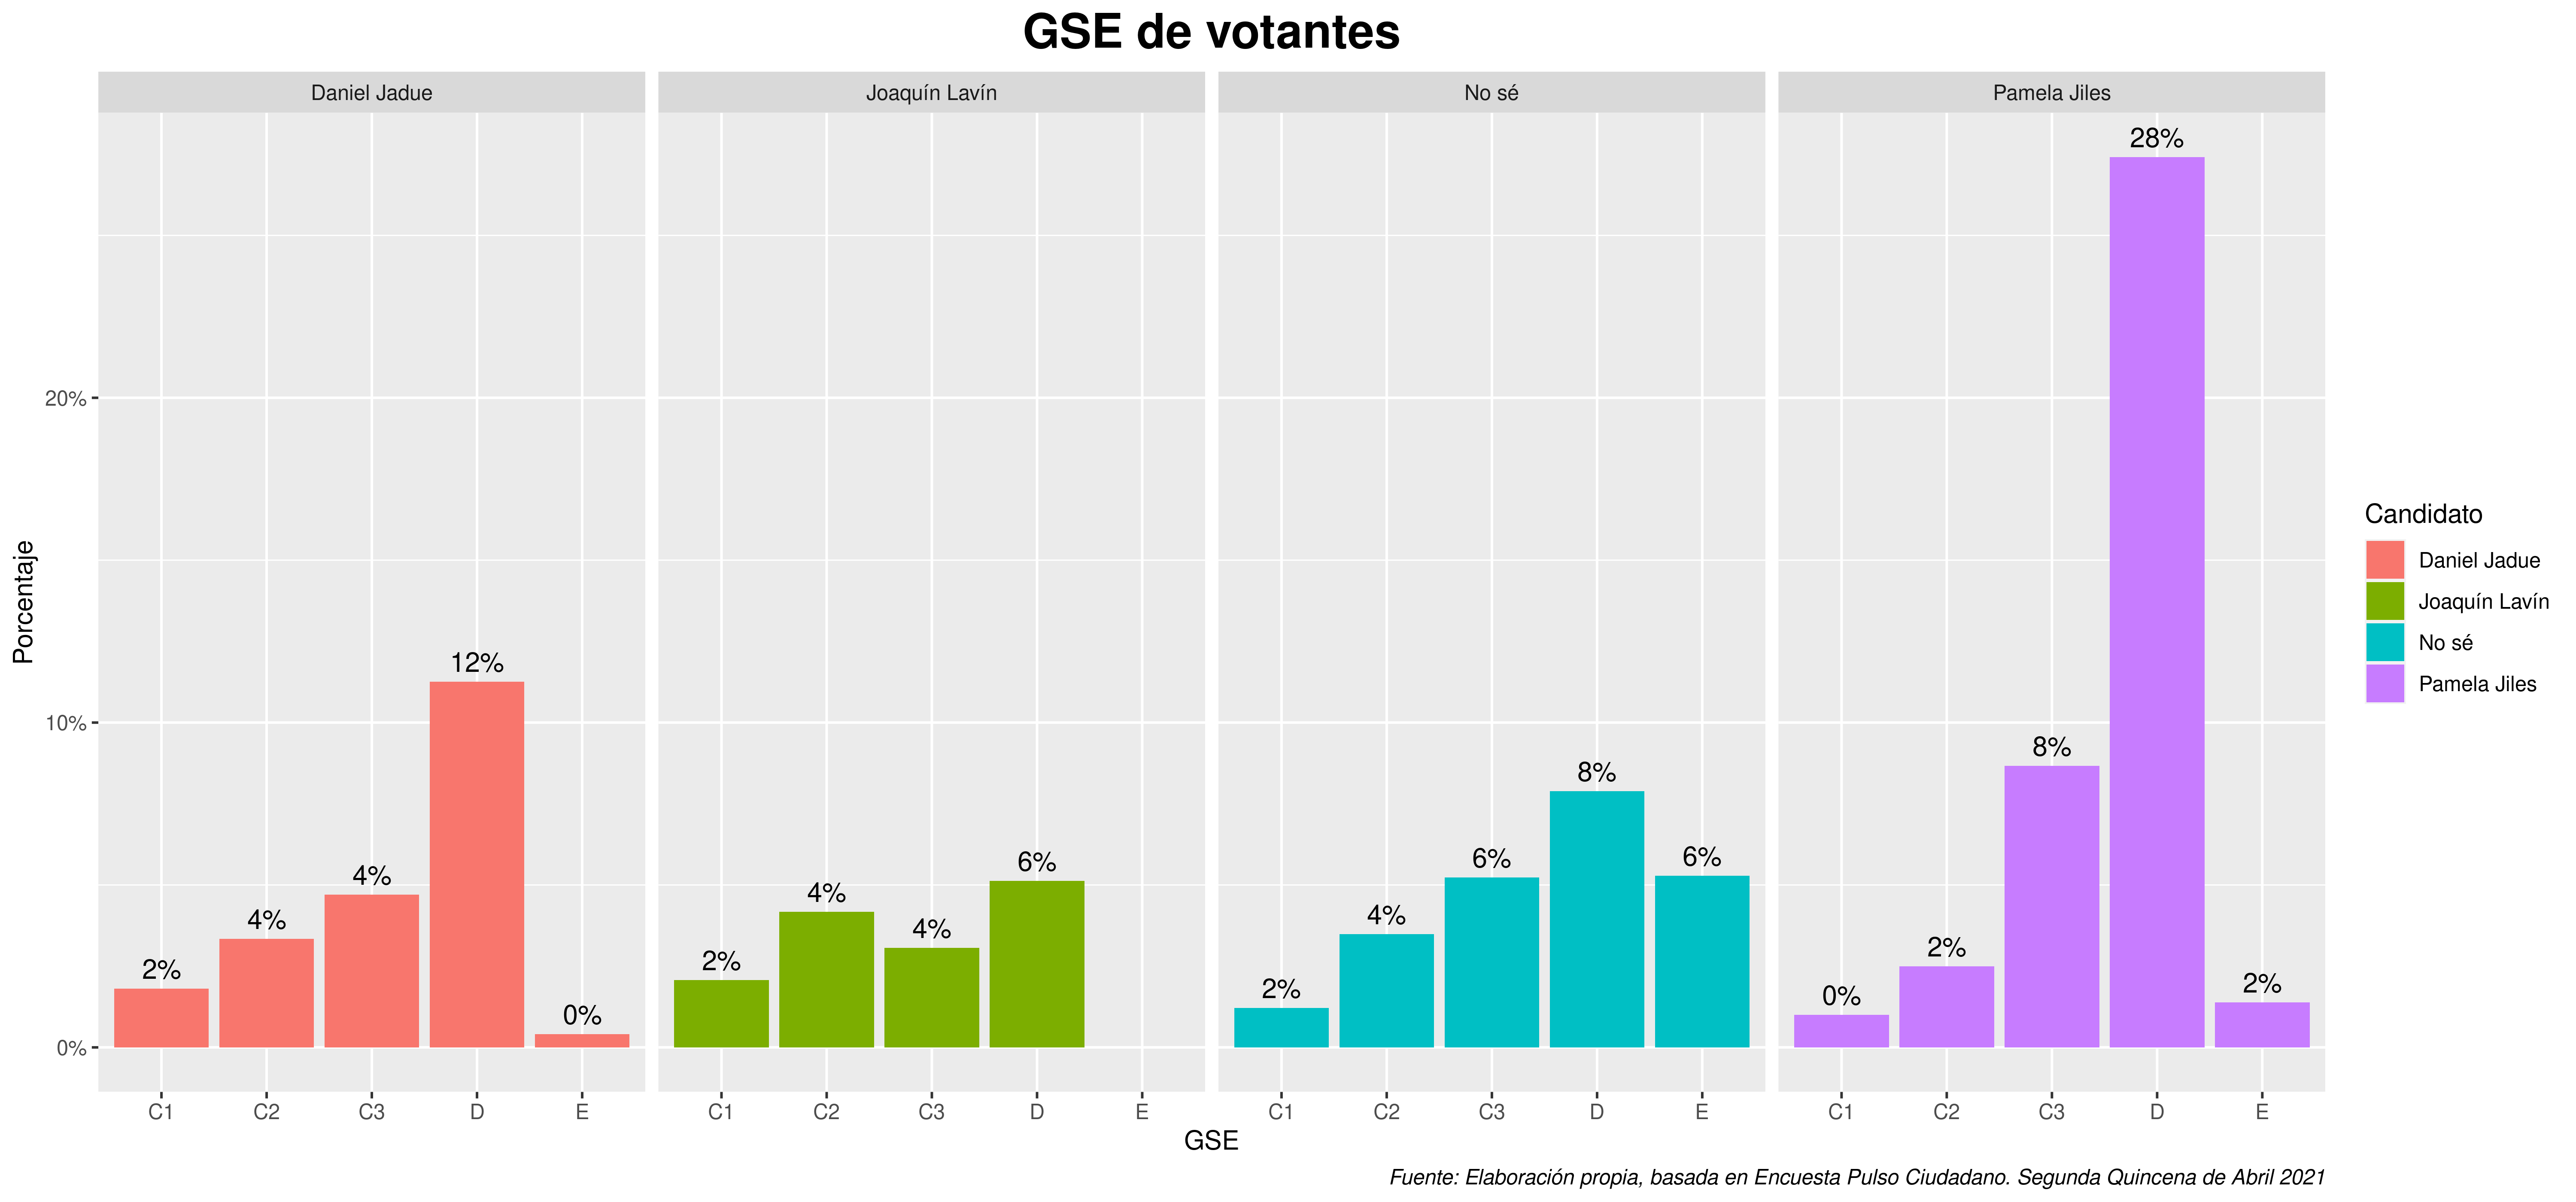
\includegraphics{GSEPlot.png} Además de observar que tanto jiles y Jadue
concentran el 40\% de los votantes que además corresponden a las clases
bajas como el sector D, es interesante observar un grupo que es el de
los que aún no sabe por quien votar. Queda todavía una gran cantidad de
personas de clase baja que aún no se deciden (probablemente más jóvenes,
donde menos ayudas económicas han llegado) pero sobre todo hay una
población dura de la clase más baja en Chile que aún no sabe por quien
votará. Este último sector, el de los más pobres, prácticamente no está
presente en ninguno de los candidatos competitivos, salvo Pamela Jiles
que tiene un 2\% del total. Es clave para cualquiera de estos candidatos
acercarse más a ese sector y a los que restan de clases más bajas.

\hypertarget{sexo}{%
\subsubsection{\texorpdfstring{\textbf{Sexo}}{Sexo}}\label{sexo}}

Desde ya un lustro el feminismo y las luchas por la destrucción del
patriarcado transformaron la política actual, y las candidaturas no son
la excepción. Desde el Frente Amplio y la Concertación han hecho una
importante cantidad de críticas hacia Daniel jadue por ``Machista'' y
``Misógino'', así como Gabriel Boric hace alardes en las noticias de
estar tomando clases de Feminismo.

Así, es necesario revisar cómo es la distribución por sexo de cada uno
de los candidatos y observar qué diferencias existen.

Observemos entonces la siguiente tabla cruzada:

\newline

\begin{longtable}[]{@{}rrrrrrr@{}}
\toprule
\endhead
\begin{minipage}[t]{0.09\columnwidth}\raggedleft
\strut
\end{minipage} & \begin{minipage}[t]{0.06\columnwidth}\raggedleft
Candi\strut
\end{minipage} & \begin{minipage}[t]{0.13\columnwidth}\raggedleft
Daniel Jadue\strut
\end{minipage} & \begin{minipage}[t]{0.12\columnwidth}\raggedleft
Joaquín Lavín\strut
\end{minipage} & \begin{minipage}[t]{0.13\columnwidth}\raggedleft
No sé\strut
\end{minipage} & \begin{minipage}[t]{0.13\columnwidth}\raggedleft
Pamela Jiles\strut
\end{minipage} & \begin{minipage}[t]{0.13\columnwidth}\raggedleft
Total\strut
\end{minipage}\tabularnewline
\begin{minipage}[t]{0.09\columnwidth}\raggedleft
SexoRecod\strut
\end{minipage} & \begin{minipage}[t]{0.06\columnwidth}\raggedleft
\strut
\end{minipage} & \begin{minipage}[t]{0.13\columnwidth}\raggedleft
\strut
\end{minipage} & \begin{minipage}[t]{0.12\columnwidth}\raggedleft
\strut
\end{minipage} & \begin{minipage}[t]{0.13\columnwidth}\raggedleft
\strut
\end{minipage} & \begin{minipage}[t]{0.13\columnwidth}\raggedleft
\strut
\end{minipage} & \begin{minipage}[t]{0.13\columnwidth}\raggedleft
\strut
\end{minipage}\tabularnewline
\begin{minipage}[t]{0.09\columnwidth}\raggedleft
hombre\strut
\end{minipage} & \begin{minipage}[t]{0.06\columnwidth}\raggedleft
\strut
\end{minipage} & \begin{minipage}[t]{0.13\columnwidth}\raggedleft
71.2 ( 58.2\%)\strut
\end{minipage} & \begin{minipage}[t]{0.12\columnwidth}\raggedleft
47.0 ( 50.8\%)\strut
\end{minipage} & \begin{minipage}[t]{0.13\columnwidth}\raggedleft
71.9 ( 41.4\%)\strut
\end{minipage} & \begin{minipage}[t]{0.13\columnwidth}\raggedleft
144.4 ( 56.3\%)\strut
\end{minipage} & \begin{minipage}[t]{0.13\columnwidth}\raggedleft
334.5 ( 51.9\%)\strut
\end{minipage}\tabularnewline
\begin{minipage}[t]{0.09\columnwidth}\raggedleft
mujer\strut
\end{minipage} & \begin{minipage}[t]{0.06\columnwidth}\raggedleft
\strut
\end{minipage} & \begin{minipage}[t]{0.13\columnwidth}\raggedleft
51.2 ( 41.8\%)\strut
\end{minipage} & \begin{minipage}[t]{0.12\columnwidth}\raggedleft
45.4 ( 49.2\%)\strut
\end{minipage} & \begin{minipage}[t]{0.13\columnwidth}\raggedleft
101.7 ( 58.6\%)\strut
\end{minipage} & \begin{minipage}[t]{0.13\columnwidth}\raggedleft
112.1 ( 43.7\%)\strut
\end{minipage} & \begin{minipage}[t]{0.13\columnwidth}\raggedleft
310.4 ( 48.1\%)\strut
\end{minipage}\tabularnewline
\begin{minipage}[t]{0.09\columnwidth}\raggedleft
Total\strut
\end{minipage} & \begin{minipage}[t]{0.06\columnwidth}\raggedleft
\strut
\end{minipage} & \begin{minipage}[t]{0.13\columnwidth}\raggedleft
122.4 (100.0\%)\strut
\end{minipage} & \begin{minipage}[t]{0.12\columnwidth}\raggedleft
92.4 (100.0\%)\strut
\end{minipage} & \begin{minipage}[t]{0.13\columnwidth}\raggedleft
173.6 (100.0\%)\strut
\end{minipage} & \begin{minipage}[t]{0.13\columnwidth}\raggedleft
256.5 (100.0\%)\strut
\end{minipage} & \begin{minipage}[t]{0.13\columnwidth}\raggedleft
644.9 (100.0\%)\strut
\end{minipage}\tabularnewline
\bottomrule
\end{longtable}

\begin{longtable}[]{@{}ccc@{}}
\toprule
\begin{minipage}[b]{0.18\columnwidth}\centering
Chi.squared\strut
\end{minipage} & \begin{minipage}[b]{0.06\columnwidth}\centering
df\strut
\end{minipage} & \begin{minipage}[b]{0.13\columnwidth}\centering
p.value\strut
\end{minipage}\tabularnewline
\midrule
\endhead
\begin{minipage}[t]{0.18\columnwidth}\centering
11.617\strut
\end{minipage} & \begin{minipage}[t]{0.06\columnwidth}\centering
3\strut
\end{minipage} & \begin{minipage}[t]{0.13\columnwidth}\centering
0.0088\strut
\end{minipage}\tabularnewline
\bottomrule
\end{longtable}

En esta tabla hay tres cosas principales a destacar. Primero: Tanto
Daniel Jadue como Pamela Jiles tienen un alto nivel de masculinización
de su voto; esto podría tener una gran cantidad de explicaciones, entre
ellas los atributos personales de ambos, pero probablemente también por
las características de los ``hombres proveedores'' que, a partir de una
distribución del patricarcado, son ellos los que más dinero tienen en la
AFP y salen a trabajar no-domésticamente para dar sustentos en sus
familias. Por otro lado Joaquín lavín está muy equilibrado en temas de
sexo.

Donde hay elementos más interesantes son en el grupo que no sabe por
quien votar: Hay una notable cantidad de mujeres aún indecisas, que no
saben por quien van a votar y que, a juzgar por las características de
los candidatos que son más competentes, no son precisamente feministas
ni necesariamente han tomado esa bandera, nisiquiera cercana a políticas
públicas centradas en las mujeres.

Probablemente la apuesta de algunos candidatos progresistas del Frente
Amplio y la concertación se estarán centrando en ese grupo de mujeres
aún indecisas, pero por lo visto sólo han fracasado.

como podemos apreciar en el gráfico que toma cada etiqueta de candidato
como una parte del 100\% de la muestra, vemos que los hombres tienen un
gran nivel de decisión de su voto, y viéndolo en perspectiva, el grupo
de indecisos están equilibrados en género, por lo que aún queda mucho
por ir a convencer para votación.

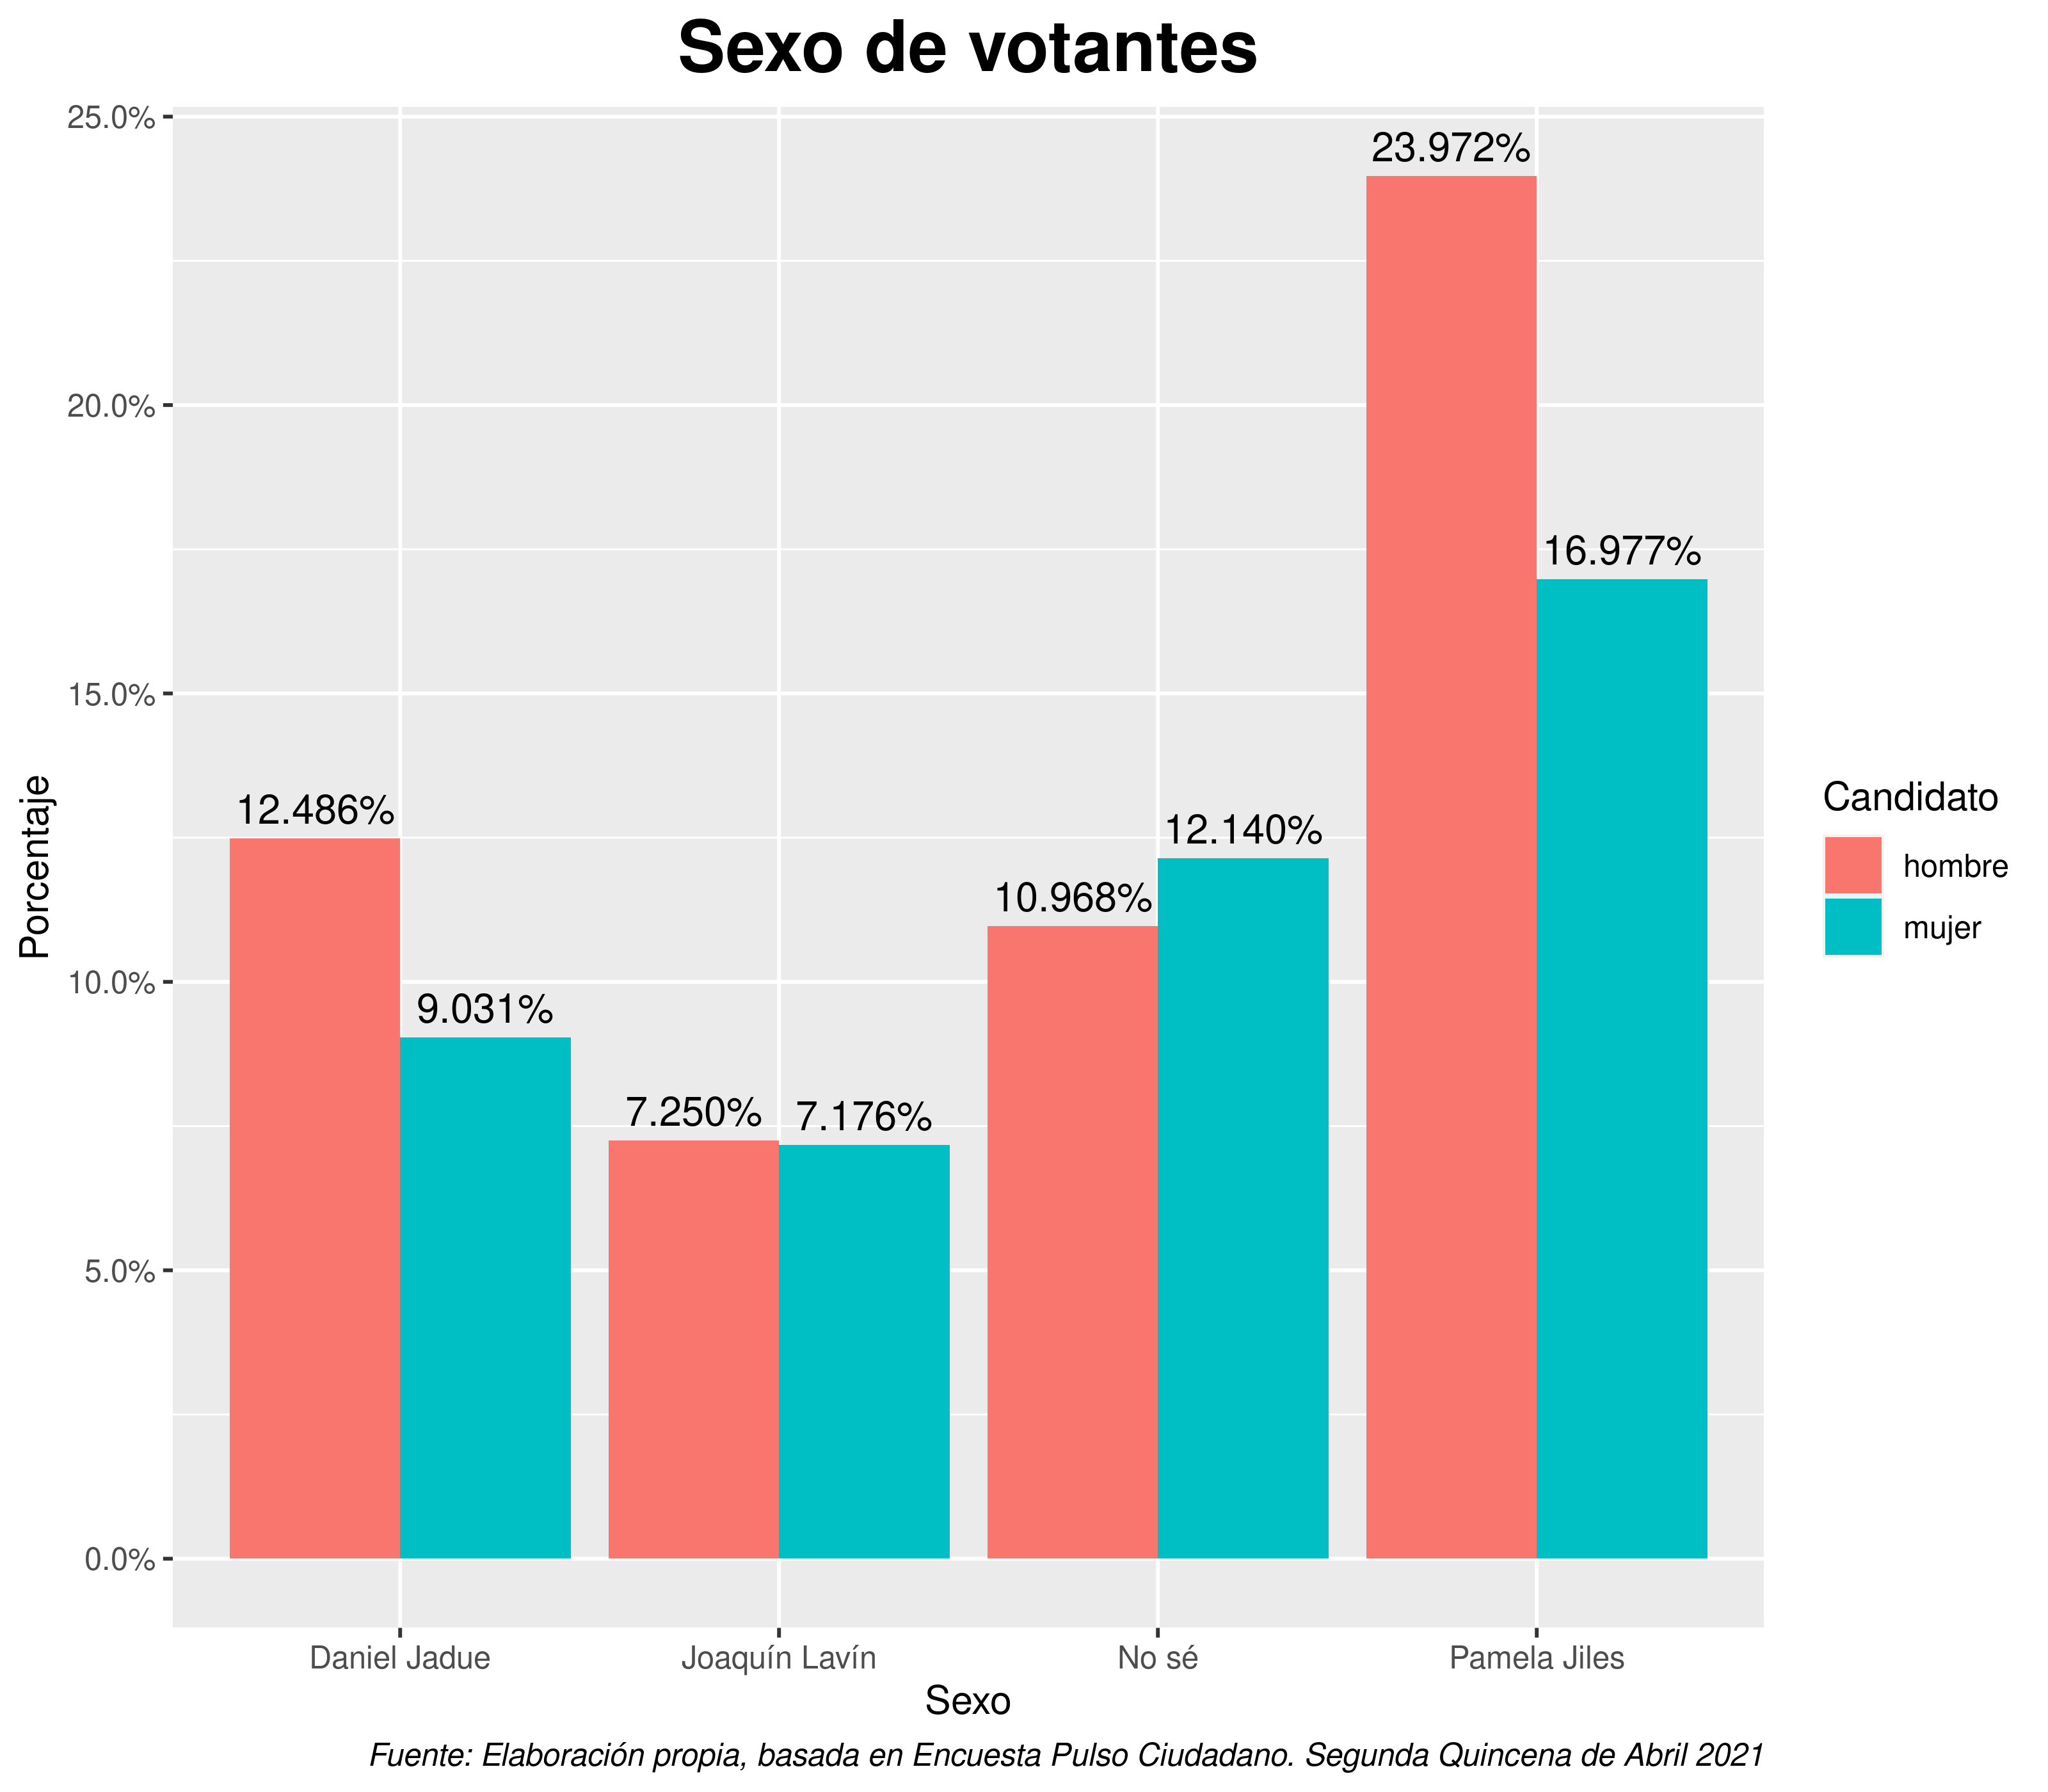
\includegraphics{SexoPlot.png}

\hypertarget{grupo-etuxe1reo}{%
\subsubsection{\texorpdfstring{\textbf{Grupo
Etáreo}}{Grupo Etáreo}}\label{grupo-etuxe1reo}}

Ahora ¿a quienes llegan más los candidatos en términos de edad? Los
grupos generacionales son bastante relevantes y ampliamente estudiados
en cómo las generaciones tienen formas distintas de socialización
política, tienen miedos y emociones diferentes, se atreven a distintas
cosas y, por sobre todo, tienen una conducta electoral diferente.

En la siguiente tabla cruzada observaremos cómo los grupos etáreos se
distribuyen en cada una de las candidaturas:

\newline

\begin{longtable}[]{@{}rrrrrrr@{}}
\toprule
\endhead
\begin{minipage}[t]{0.11\columnwidth}\raggedleft
\strut
\end{minipage} & \begin{minipage}[t]{0.06\columnwidth}\raggedleft
Candi\strut
\end{minipage} & \begin{minipage}[t]{0.13\columnwidth}\raggedleft
Daniel Jadue\strut
\end{minipage} & \begin{minipage}[t]{0.12\columnwidth}\raggedleft
Joaquín Lavín\strut
\end{minipage} & \begin{minipage}[t]{0.13\columnwidth}\raggedleft
No sé\strut
\end{minipage} & \begin{minipage}[t]{0.13\columnwidth}\raggedleft
Pamela Jiles\strut
\end{minipage} & \begin{minipage}[t]{0.13\columnwidth}\raggedleft
Total\strut
\end{minipage}\tabularnewline
\begin{minipage}[t]{0.11\columnwidth}\raggedleft
Edadrec\strut
\end{minipage} & \begin{minipage}[t]{0.06\columnwidth}\raggedleft
\strut
\end{minipage} & \begin{minipage}[t]{0.13\columnwidth}\raggedleft
\strut
\end{minipage} & \begin{minipage}[t]{0.12\columnwidth}\raggedleft
\strut
\end{minipage} & \begin{minipage}[t]{0.13\columnwidth}\raggedleft
\strut
\end{minipage} & \begin{minipage}[t]{0.13\columnwidth}\raggedleft
\strut
\end{minipage} & \begin{minipage}[t]{0.13\columnwidth}\raggedleft
\strut
\end{minipage}\tabularnewline
\begin{minipage}[t]{0.11\columnwidth}\raggedleft
Boomers\strut
\end{minipage} & \begin{minipage}[t]{0.06\columnwidth}\raggedleft
\strut
\end{minipage} & \begin{minipage}[t]{0.13\columnwidth}\raggedleft
39.3 ( 32.1\%)\strut
\end{minipage} & \begin{minipage}[t]{0.12\columnwidth}\raggedleft
24.6 ( 26.6\%)\strut
\end{minipage} & \begin{minipage}[t]{0.13\columnwidth}\raggedleft
50.9 ( 29.3\%)\strut
\end{minipage} & \begin{minipage}[t]{0.13\columnwidth}\raggedleft
117.9 ( 45.9\%)\strut
\end{minipage} & \begin{minipage}[t]{0.13\columnwidth}\raggedleft
232.6 ( 36.1\%)\strut
\end{minipage}\tabularnewline
\begin{minipage}[t]{0.11\columnwidth}\raggedleft
Centennials\strut
\end{minipage} & \begin{minipage}[t]{0.06\columnwidth}\raggedleft
\strut
\end{minipage} & \begin{minipage}[t]{0.13\columnwidth}\raggedleft
5.7 ( 4.6\%)\strut
\end{minipage} & \begin{minipage}[t]{0.12\columnwidth}\raggedleft
9.3 ( 10.1\%)\strut
\end{minipage} & \begin{minipage}[t]{0.13\columnwidth}\raggedleft
28.7 ( 16.5\%)\strut
\end{minipage} & \begin{minipage}[t]{0.13\columnwidth}\raggedleft
6.3 ( 2.5\%)\strut
\end{minipage} & \begin{minipage}[t]{0.13\columnwidth}\raggedleft
50.0 ( 7.8\%)\strut
\end{minipage}\tabularnewline
\begin{minipage}[t]{0.11\columnwidth}\raggedleft
Gen X\strut
\end{minipage} & \begin{minipage}[t]{0.06\columnwidth}\raggedleft
\strut
\end{minipage} & \begin{minipage}[t]{0.13\columnwidth}\raggedleft
30.2 ( 24.7\%)\strut
\end{minipage} & \begin{minipage}[t]{0.12\columnwidth}\raggedleft
27.3 ( 29.6\%)\strut
\end{minipage} & \begin{minipage}[t]{0.13\columnwidth}\raggedleft
55.9 ( 32.2\%)\strut
\end{minipage} & \begin{minipage}[t]{0.13\columnwidth}\raggedleft
60.9 ( 23.7\%)\strut
\end{minipage} & \begin{minipage}[t]{0.13\columnwidth}\raggedleft
174.3 ( 27.0\%)\strut
\end{minipage}\tabularnewline
\begin{minipage}[t]{0.11\columnwidth}\raggedleft
Millennials\strut
\end{minipage} & \begin{minipage}[t]{0.06\columnwidth}\raggedleft
\strut
\end{minipage} & \begin{minipage}[t]{0.13\columnwidth}\raggedleft
47.2 ( 38.6\%)\strut
\end{minipage} & \begin{minipage}[t]{0.12\columnwidth}\raggedleft
31.1 ( 33.7\%)\strut
\end{minipage} & \begin{minipage}[t]{0.13\columnwidth}\raggedleft
38.1 ( 21.9\%)\strut
\end{minipage} & \begin{minipage}[t]{0.13\columnwidth}\raggedleft
71.5 ( 27.9\%)\strut
\end{minipage} & \begin{minipage}[t]{0.13\columnwidth}\raggedleft
187.9 ( 29.1\%)\strut
\end{minipage}\tabularnewline
\begin{minipage}[t]{0.11\columnwidth}\raggedleft
Total\strut
\end{minipage} & \begin{minipage}[t]{0.06\columnwidth}\raggedleft
\strut
\end{minipage} & \begin{minipage}[t]{0.13\columnwidth}\raggedleft
122.4 (100.0\%)\strut
\end{minipage} & \begin{minipage}[t]{0.12\columnwidth}\raggedleft
92.4 (100.0\%)\strut
\end{minipage} & \begin{minipage}[t]{0.13\columnwidth}\raggedleft
173.6 (100.0\%)\strut
\end{minipage} & \begin{minipage}[t]{0.13\columnwidth}\raggedleft
256.5 (100.0\%)\strut
\end{minipage} & \begin{minipage}[t]{0.13\columnwidth}\raggedleft
644.9 (100.0\%)\strut
\end{minipage}\tabularnewline
\bottomrule
\end{longtable}

\begin{longtable}[]{@{}ccc@{}}
\toprule
\begin{minipage}[b]{0.18\columnwidth}\centering
Chi.squared\strut
\end{minipage} & \begin{minipage}[b]{0.06\columnwidth}\centering
df\strut
\end{minipage} & \begin{minipage}[b]{0.13\columnwidth}\centering
p.value\strut
\end{minipage}\tabularnewline
\midrule
\endhead
\begin{minipage}[t]{0.18\columnwidth}\centering
51.4222\strut
\end{minipage} & \begin{minipage}[t]{0.06\columnwidth}\centering
9\strut
\end{minipage} & \begin{minipage}[t]{0.13\columnwidth}\centering
0\strut
\end{minipage}\tabularnewline
\bottomrule
\end{longtable}

A pesar de que Pamela Jiles haya hecho una de sus performances como
Naruto (y muy mal interpretadas por un Diputado de derecha), uno
pensaría que ella es por lejos una de las personas que debería tener
cautivos a la gente joven, pero la verdad es que Jiles pareciera tener
\emph{nulo interés por los grupos más jóvenes}; en otras palabras, jiles
es un eminente fenómeno para personas mayores, con casi la mitad de su
votación, y que claramente esto se debe a los procesos de retiros de
fondos de las AFP, del cual casi lleva un año.

Por otro lado Daniel Jadue tiene un muy notable arraigo en generaciones
adulto jóvenes y adultas, sobre todo Gen X (36 -51 años) y Millenials
(22 -35 años); es probable que en este ámbito haya una amplia
correlación con niveles educativos más altos, dado el carácter
doctrinario/ideológico que implica Jadue, pero esto quedará en pura
especulación con preguntas que no existen.

Por otro ladpo joaquín Lavin pareciera ser relativamente homogéneo, pero
llama la atención que el sector de centenialls (18 a 21 años, para
efectos de la encuesta) es más alto que en los otros candidatos.

Para hablar del último grupo de los que aún no saben, observemos un poco
más el gráfico con la totalidad:

\newline

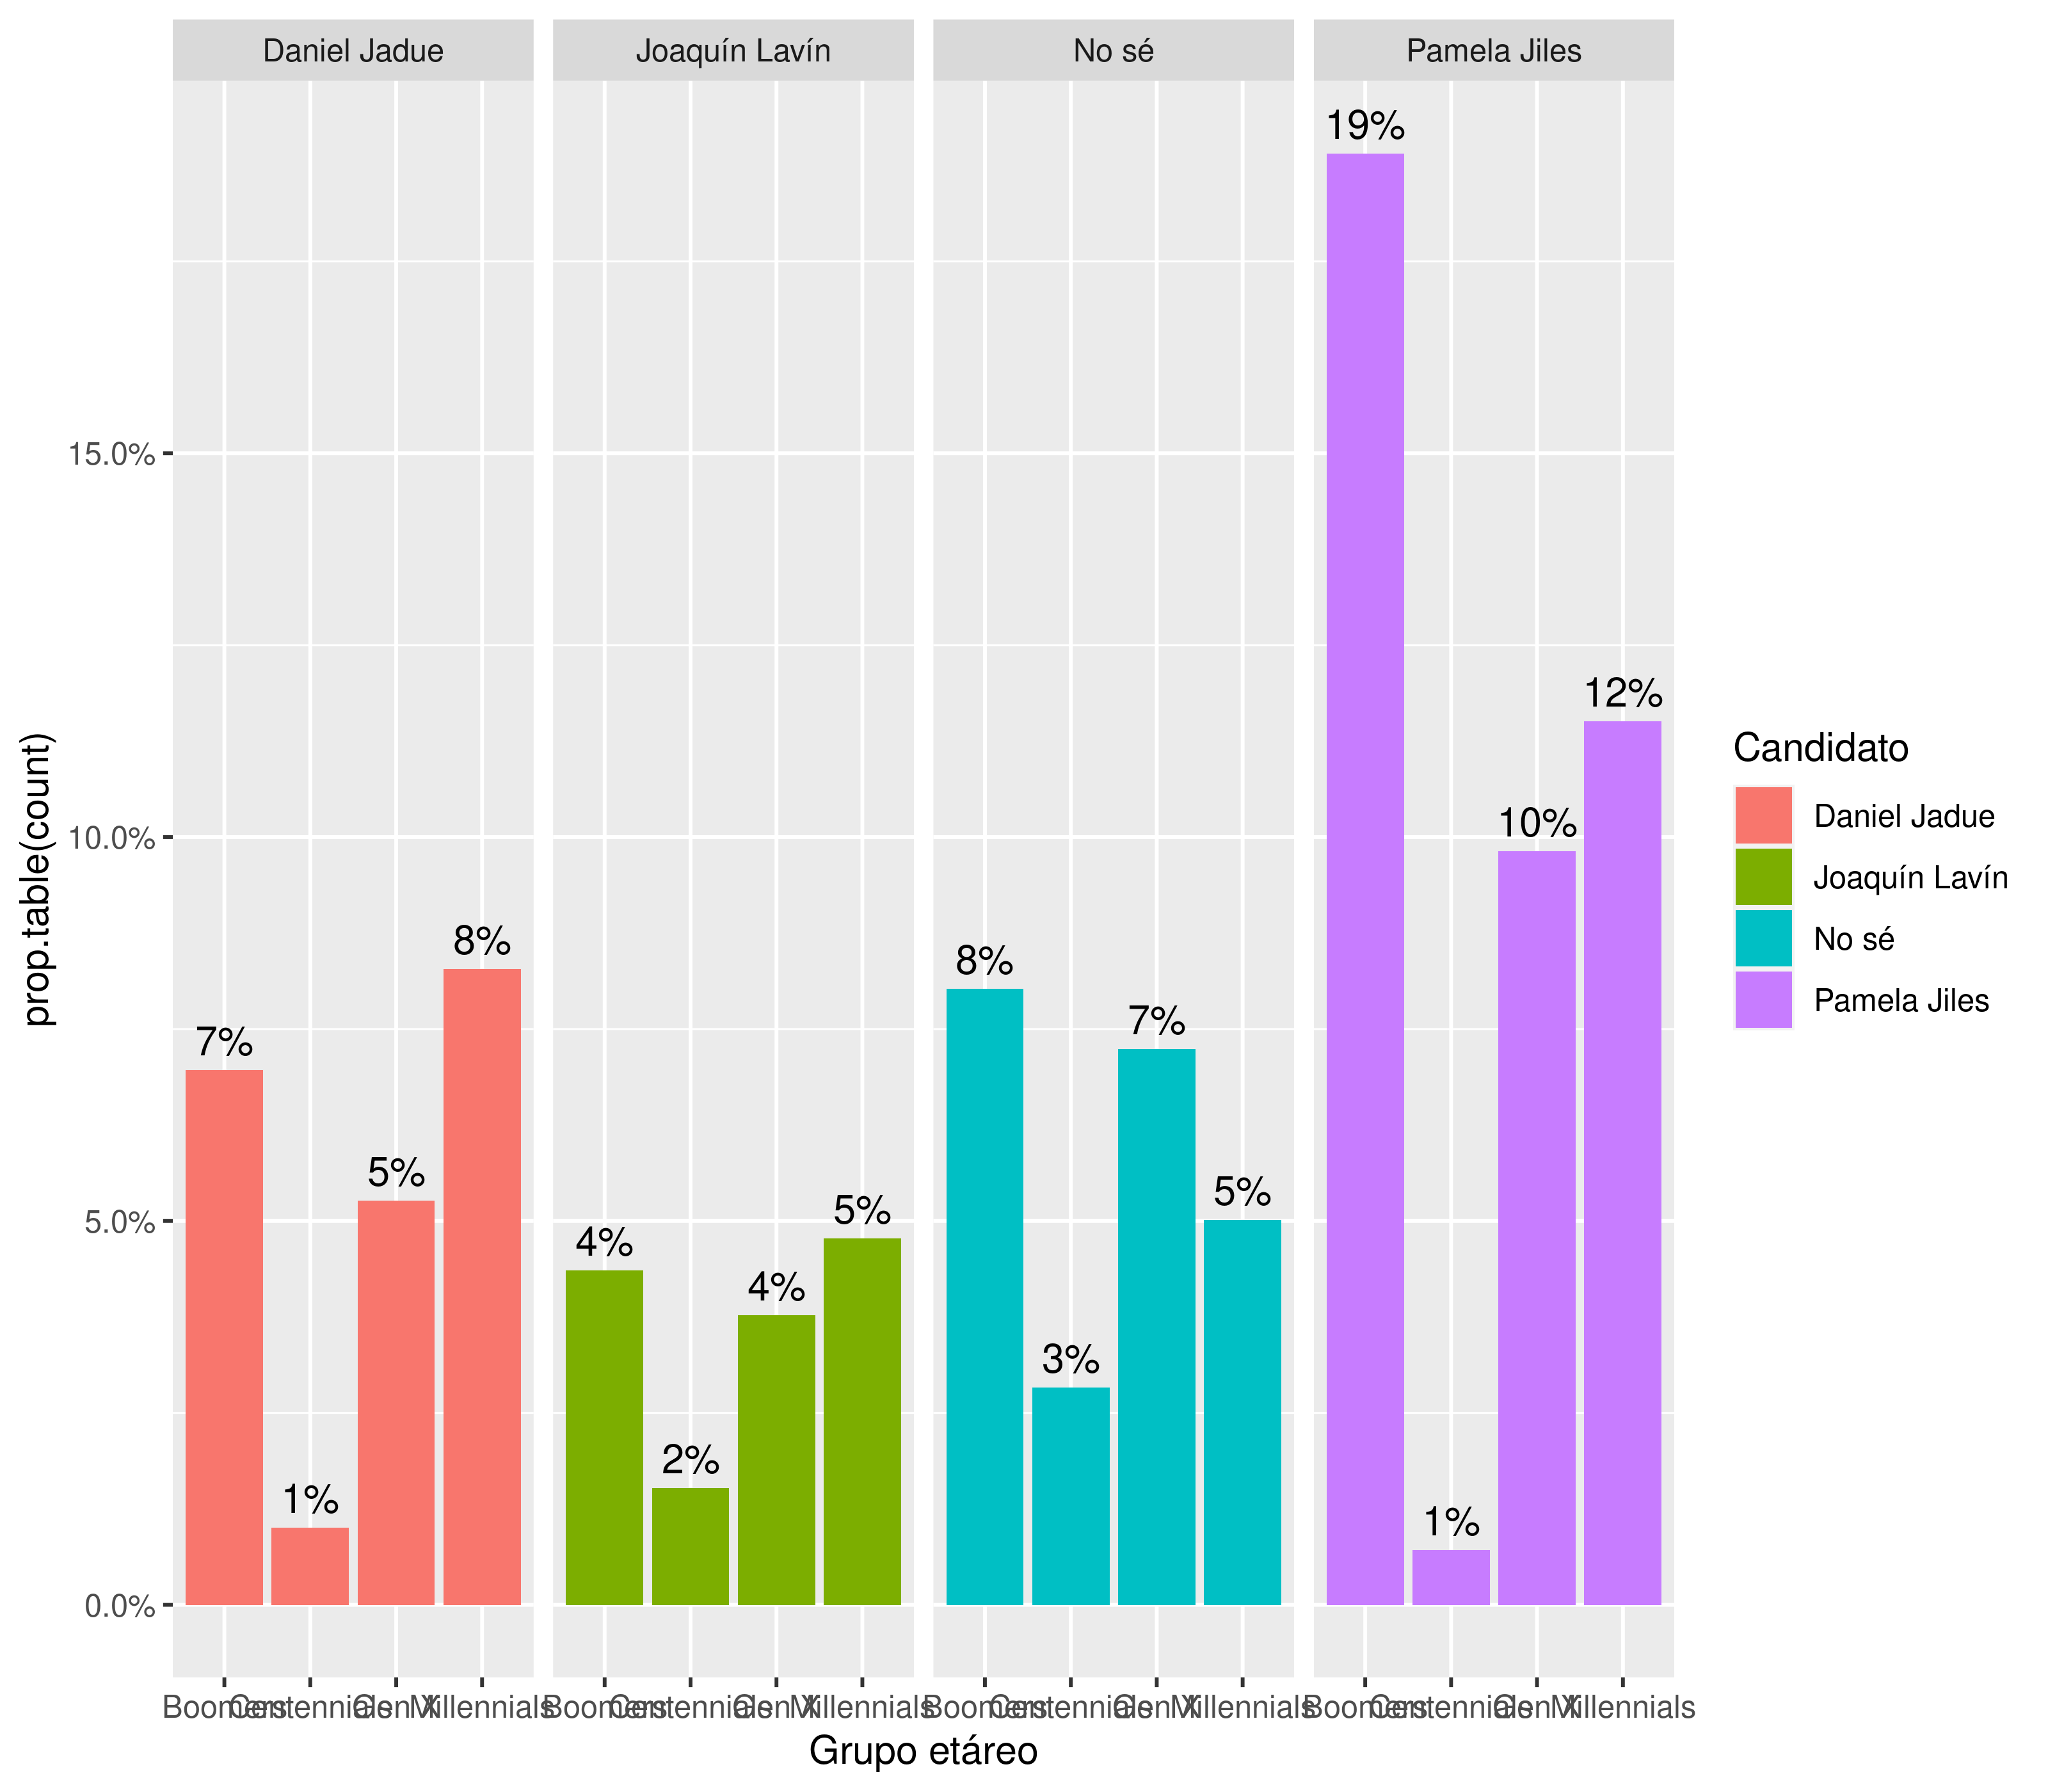
\includegraphics{EdadPlot.png} \newline

Podemos señalar que existe aún un ``bolsón de votantes'' aún indecisos
marcados polarmente por las edades: los boomer (más de 52 años) con un
8\% del total de indecisos, y los Centenialls (18 a 21 años) con un 7\%
de posibles votantes. Sugeriría ponerle atención a estos grupos y y
adoptar mecanismos y políticas publicas enfocadas en ellos, sobre todo
porque las ayudas económicas y fenómenos como la educación sólo han
sabido de humillación para estos sectores, incluídos además la exclusión
del proceso constiuyente de los más jóvenes.

\newline

\hypertarget{situaciuxf3n-econuxf3mica-de-quienes-votan}{%
\subsection{\texorpdfstring{\textbf{Situación económica de quienes
votan}}{Situación económica de quienes votan}}\label{situaciuxf3n-econuxf3mica-de-quienes-votan}}

Similar a lo que implica la estratificación social y económica según los
votantes, actualmente la situación laboral y el dinero que ganan es un
argumento cada vesz más poderosoque puede condicionar la conducta
electoral en el país, sobre todo con los niveles de pobreza actual. Esta
misma encuesta Pulso Ciudadano hubica, según GSE, los niveles de
cesantía entre 33\% (en el caso de los sectores D y E) hasta el 12\% de
cesantía en el sector C1.

Analicemos, pues, los datos que dan tanto la tabla como el gráfico.

\begin{longtable}[]{@{}rrrrrrr@{}}
\toprule
\endhead
\begin{minipage}[t]{0.15\columnwidth}\raggedleft
\strut
\end{minipage} & \begin{minipage}[t]{0.05\columnwidth}\raggedleft
Candi\strut
\end{minipage} & \begin{minipage}[t]{0.12\columnwidth}\raggedleft
Daniel Jadue\strut
\end{minipage} & \begin{minipage}[t]{0.11\columnwidth}\raggedleft
Joaquín Lavín\strut
\end{minipage} & \begin{minipage}[t]{0.12\columnwidth}\raggedleft
No sé\strut
\end{minipage} & \begin{minipage}[t]{0.12\columnwidth}\raggedleft
Pamela Jiles\strut
\end{minipage} & \begin{minipage}[t]{0.12\columnwidth}\raggedleft
Total\strut
\end{minipage}\tabularnewline
\begin{minipage}[t]{0.15\columnwidth}\raggedleft
Labor\strut
\end{minipage} & \begin{minipage}[t]{0.05\columnwidth}\raggedleft
\strut
\end{minipage} & \begin{minipage}[t]{0.12\columnwidth}\raggedleft
\strut
\end{minipage} & \begin{minipage}[t]{0.11\columnwidth}\raggedleft
\strut
\end{minipage} & \begin{minipage}[t]{0.12\columnwidth}\raggedleft
\strut
\end{minipage} & \begin{minipage}[t]{0.12\columnwidth}\raggedleft
\strut
\end{minipage} & \begin{minipage}[t]{0.12\columnwidth}\raggedleft
\strut
\end{minipage}\tabularnewline
\begin{minipage}[t]{0.15\columnwidth}\raggedleft
Cesante\strut
\end{minipage} & \begin{minipage}[t]{0.05\columnwidth}\raggedleft
\strut
\end{minipage} & \begin{minipage}[t]{0.12\columnwidth}\raggedleft
25.4 ( 20.9\%)\strut
\end{minipage} & \begin{minipage}[t]{0.11\columnwidth}\raggedleft
18.8 ( 23.1\%)\strut
\end{minipage} & \begin{minipage}[t]{0.12\columnwidth}\raggedleft
28.0 ( 21.5\%)\strut
\end{minipage} & \begin{minipage}[t]{0.12\columnwidth}\raggedleft
68.5 ( 29.6\%)\strut
\end{minipage} & \begin{minipage}[t]{0.12\columnwidth}\raggedleft
140.6 ( 24.9\%)\strut
\end{minipage}\tabularnewline
\begin{minipage}[t]{0.15\columnwidth}\raggedleft
Jefe de Hogar\strut
\end{minipage} & \begin{minipage}[t]{0.05\columnwidth}\raggedleft
\strut
\end{minipage} & \begin{minipage}[t]{0.12\columnwidth}\raggedleft
4.8 ( 4.0\%)\strut
\end{minipage} & \begin{minipage}[t]{0.11\columnwidth}\raggedleft
15.8 ( 19.4\%)\strut
\end{minipage} & \begin{minipage}[t]{0.12\columnwidth}\raggedleft
27.4 ( 21.0\%)\strut
\end{minipage} & \begin{minipage}[t]{0.12\columnwidth}\raggedleft
25.3 ( 11.0\%)\strut
\end{minipage} & \begin{minipage}[t]{0.12\columnwidth}\raggedleft
73.3 ( 13.0\%)\strut
\end{minipage}\tabularnewline
\begin{minipage}[t]{0.15\columnwidth}\raggedleft
Jubilado\strut
\end{minipage} & \begin{minipage}[t]{0.05\columnwidth}\raggedleft
\strut
\end{minipage} & \begin{minipage}[t]{0.12\columnwidth}\raggedleft
5.3 ( 4.4\%)\strut
\end{minipage} & \begin{minipage}[t]{0.11\columnwidth}\raggedleft
1.3 ( 1.6\%)\strut
\end{minipage} & \begin{minipage}[t]{0.12\columnwidth}\raggedleft
7.2 ( 5.5\%)\strut
\end{minipage} & \begin{minipage}[t]{0.12\columnwidth}\raggedleft
26.2 ( 11.4\%)\strut
\end{minipage} & \begin{minipage}[t]{0.12\columnwidth}\raggedleft
40.1 ( 7.1\%)\strut
\end{minipage}\tabularnewline
\begin{minipage}[t]{0.15\columnwidth}\raggedleft
Sólo estudiando\strut
\end{minipage} & \begin{minipage}[t]{0.05\columnwidth}\raggedleft
\strut
\end{minipage} & \begin{minipage}[t]{0.12\columnwidth}\raggedleft
12.6 ( 10.4\%)\strut
\end{minipage} & \begin{minipage}[t]{0.11\columnwidth}\raggedleft
7.2 ( 8.9\%)\strut
\end{minipage} & \begin{minipage}[t]{0.12\columnwidth}\raggedleft
14.8 ( 11.3\%)\strut
\end{minipage} & \begin{minipage}[t]{0.12\columnwidth}\raggedleft
4.7 ( 2.0\%)\strut
\end{minipage} & \begin{minipage}[t]{0.12\columnwidth}\raggedleft
39.3 ( 7.0\%)\strut
\end{minipage}\tabularnewline
\begin{minipage}[t]{0.15\columnwidth}\raggedleft
Teletrabajo\strut
\end{minipage} & \begin{minipage}[t]{0.05\columnwidth}\raggedleft
\strut
\end{minipage} & \begin{minipage}[t]{0.12\columnwidth}\raggedleft
33.8 ( 27.8\%)\strut
\end{minipage} & \begin{minipage}[t]{0.11\columnwidth}\raggedleft
11.2 ( 13.8\%)\strut
\end{minipage} & \begin{minipage}[t]{0.12\columnwidth}\raggedleft
24.5 ( 18.8\%)\strut
\end{minipage} & \begin{minipage}[t]{0.12\columnwidth}\raggedleft
18.5 ( 8.0\%)\strut
\end{minipage} & \begin{minipage}[t]{0.12\columnwidth}\raggedleft
87.9 ( 15.6\%)\strut
\end{minipage}\tabularnewline
\begin{minipage}[t]{0.15\columnwidth}\raggedleft
Trabajo presencial\strut
\end{minipage} & \begin{minipage}[t]{0.05\columnwidth}\raggedleft
\strut
\end{minipage} & \begin{minipage}[t]{0.12\columnwidth}\raggedleft
39.5 ( 32.6\%)\strut
\end{minipage} & \begin{minipage}[t]{0.11\columnwidth}\raggedleft
27.0 ( 33.2\%)\strut
\end{minipage} & \begin{minipage}[t]{0.12\columnwidth}\raggedleft
28.6 ( 21.9\%)\strut
\end{minipage} & \begin{minipage}[t]{0.12\columnwidth}\raggedleft
87.8 ( 38.0\%)\strut
\end{minipage} & \begin{minipage}[t]{0.12\columnwidth}\raggedleft
182.9 ( 32.4\%)\strut
\end{minipage}\tabularnewline
\begin{minipage}[t]{0.15\columnwidth}\raggedleft
Total\strut
\end{minipage} & \begin{minipage}[t]{0.05\columnwidth}\raggedleft
\strut
\end{minipage} & \begin{minipage}[t]{0.12\columnwidth}\raggedleft
121.4 (100.0\%)\strut
\end{minipage} & \begin{minipage}[t]{0.11\columnwidth}\raggedleft
81.4 (100.0\%)\strut
\end{minipage} & \begin{minipage}[t]{0.12\columnwidth}\raggedleft
130.4 (100.0\%)\strut
\end{minipage} & \begin{minipage}[t]{0.12\columnwidth}\raggedleft
231.0 (100.0\%)\strut
\end{minipage} & \begin{minipage}[t]{0.12\columnwidth}\raggedleft
564.2 (100.0\%)\strut
\end{minipage}\tabularnewline
\bottomrule
\end{longtable}

\begin{longtable}[]{@{}ccc@{}}
\toprule
\begin{minipage}[b]{0.18\columnwidth}\centering
Chi.squared\strut
\end{minipage} & \begin{minipage}[b]{0.06\columnwidth}\centering
df\strut
\end{minipage} & \begin{minipage}[b]{0.13\columnwidth}\centering
p.value\strut
\end{minipage}\tabularnewline
\midrule
\endhead
\begin{minipage}[t]{0.18\columnwidth}\centering
74.0474\strut
\end{minipage} & \begin{minipage}[t]{0.06\columnwidth}\centering
15\strut
\end{minipage} & \begin{minipage}[t]{0.13\columnwidth}\centering
0\strut
\end{minipage}\tabularnewline
\bottomrule
\end{longtable}

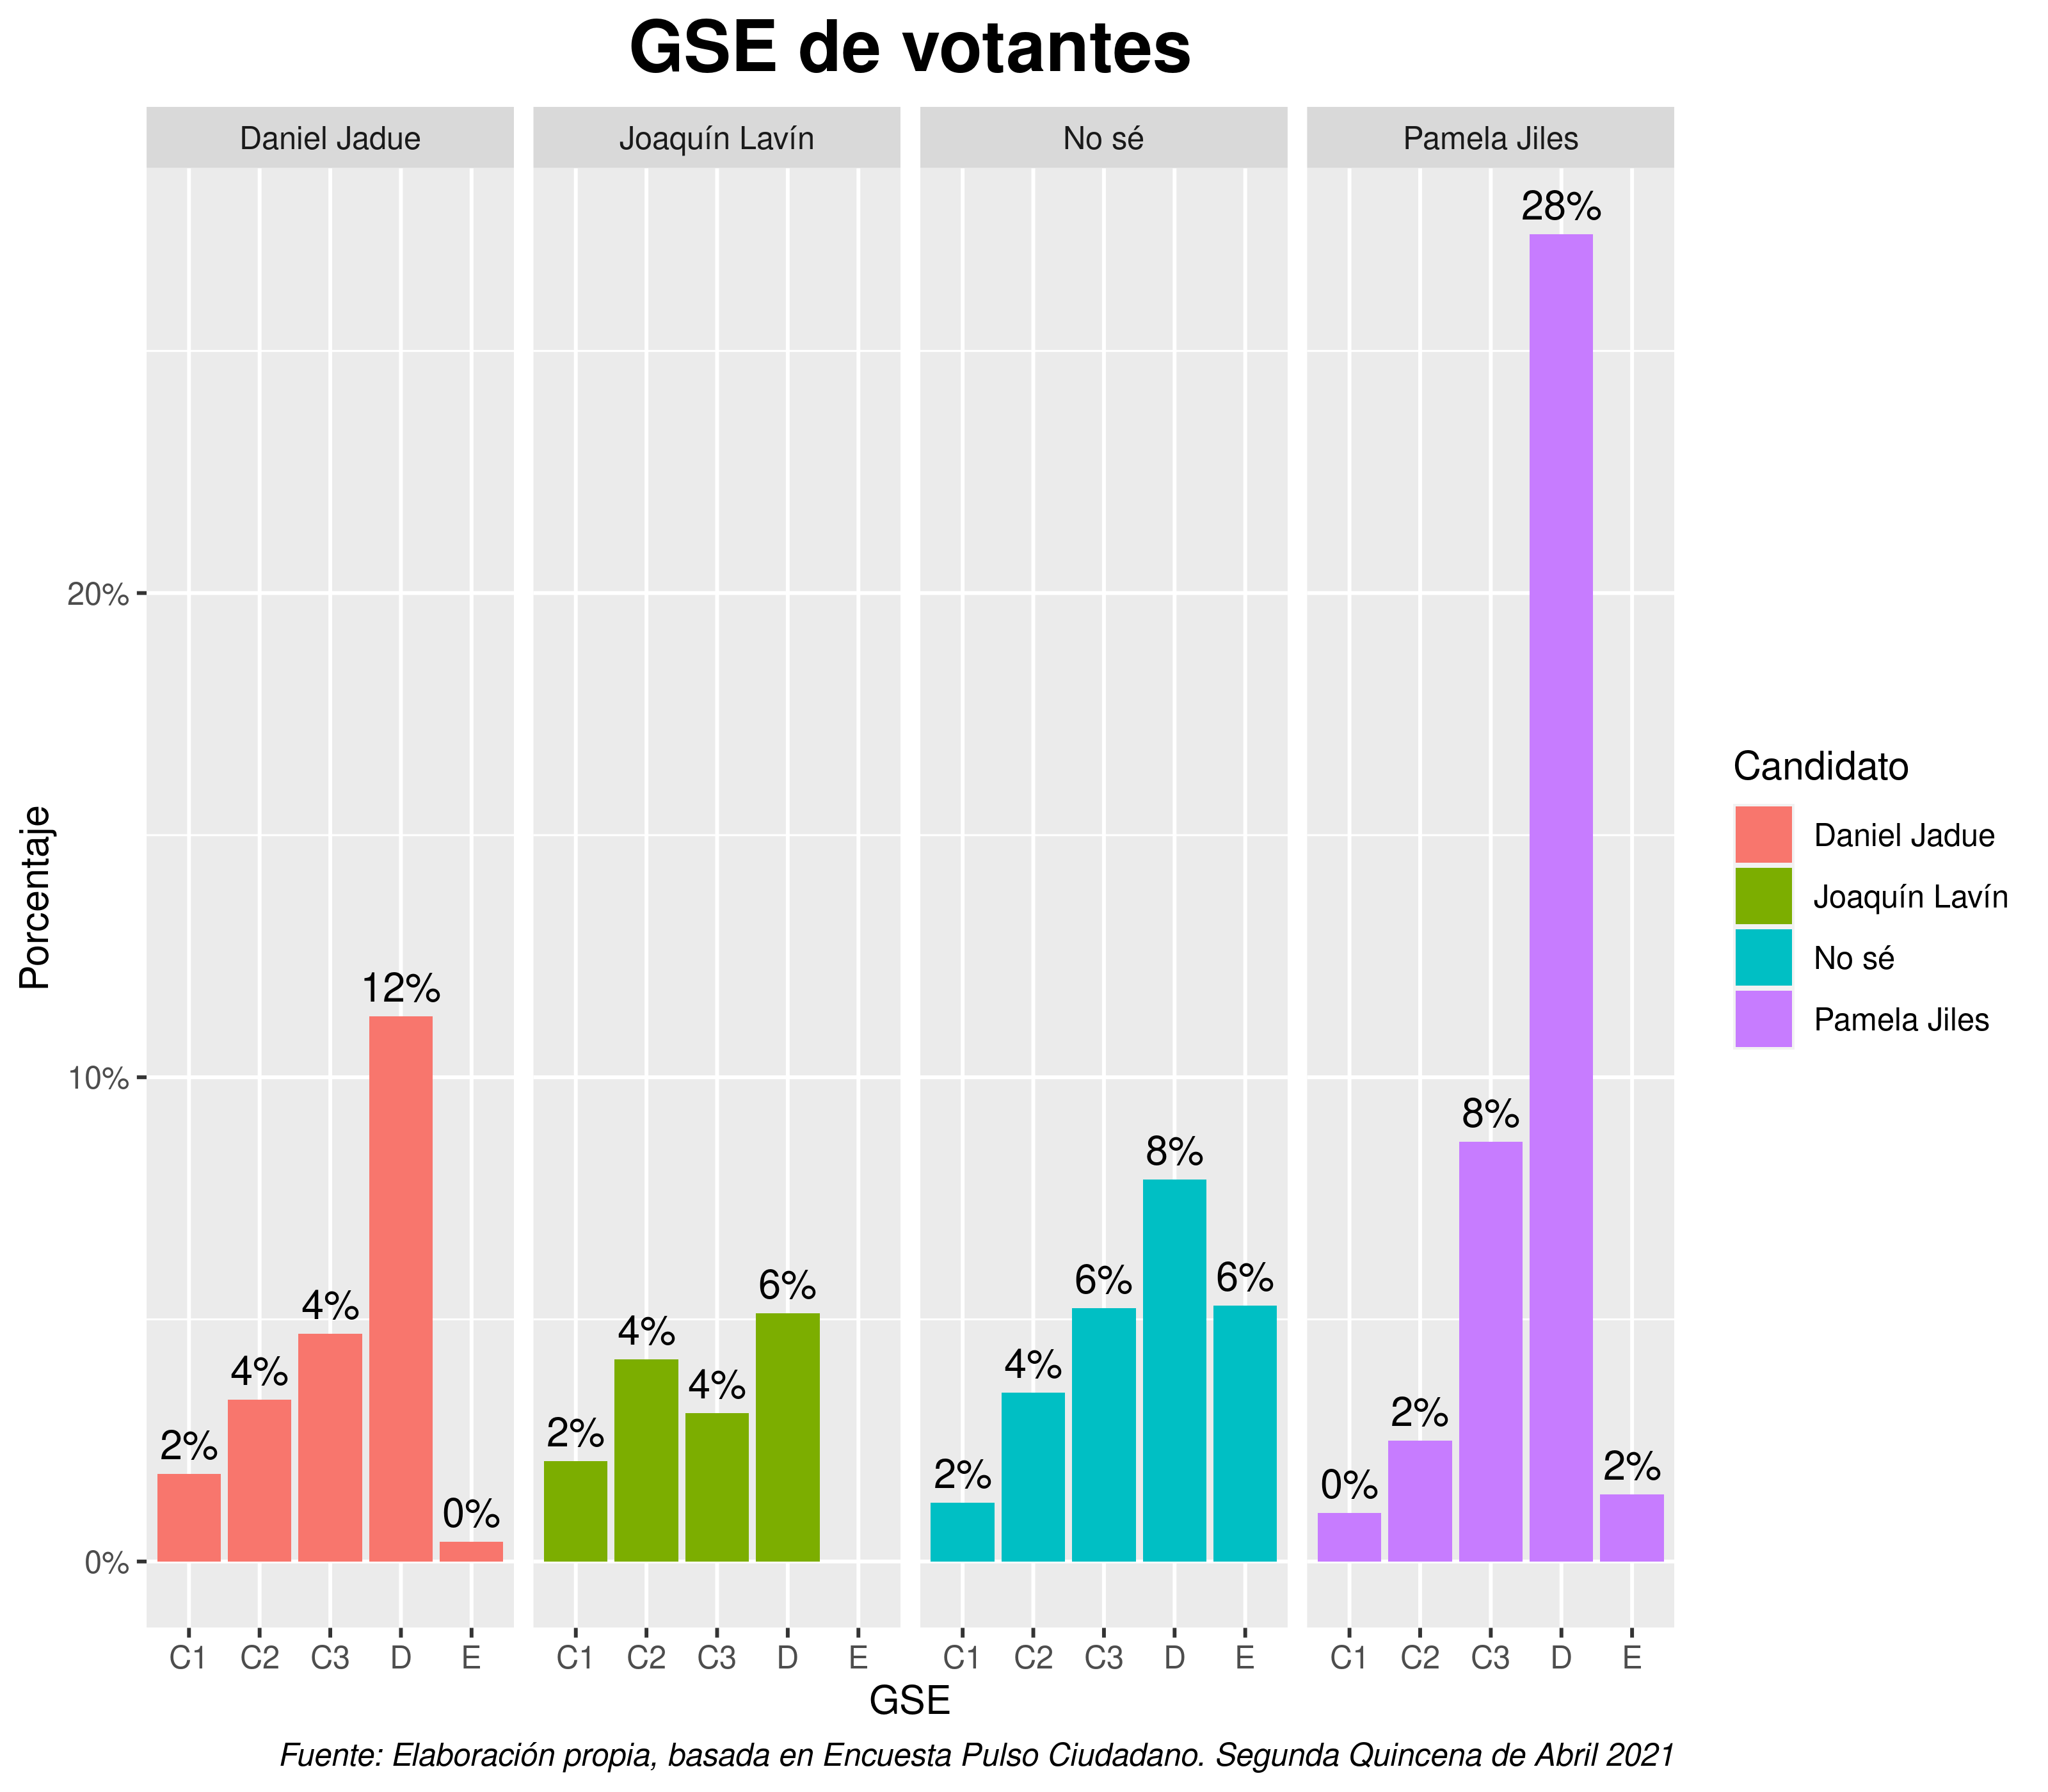
\includegraphics{LaborPlot.png} Analistas políticos/electorales de
derecha como Gonzalo Müller adscriben a la tesis de que el fenómeno de
Pamela Jiles es más bien un fenómeno de clases medias y no de sus
\emph{Sin Monea}, sin embargo considerando los GSE y esta información,
vemos que son más bien un fenómeno de \emph{trabajadores pobres}: gente
que trabaja y/o teletrabaja pero que se mantiene en sectores muy bajos,
además de casi un 30\% de personas cesantes que votan por ella, el
porcentaje más alto de cualquiera de los otros candidatos. En resumen,
Müller se equivoca rotundamente.

Por otro lado, Daniel Jadue tiene una distribución que considero
``sorpresiva'': Una alta cantidad de estudiantes que votarían
eventualmente por él (ahí relaciona el nivel educacional del cuál
hablaba anteriormente), una porción no menor de cesantes aunque a 10
puntos porcentuales de Jiles; finalmente, más de la mitad de sus
votantes se encuentran trabajando y teletrabajando.

Finalmente, sería interesante hipotetizar las diferencias entre
teletrabajo v/s trabajo presencial. ¿Significará el trabajo presencial
trabajo precarizado? Si es así, Jiles tiene una cantidad importante de
votantes de este tipo.

\begin{longtable}[]{@{}rrrrrrr@{}}
\toprule
\endhead
\begin{minipage}[t]{0.13\columnwidth}\raggedleft
\strut
\end{minipage} & \begin{minipage}[t]{0.05\columnwidth}\raggedleft
Candi\strut
\end{minipage} & \begin{minipage}[t]{0.13\columnwidth}\raggedleft
Daniel Jadue\strut
\end{minipage} & \begin{minipage}[t]{0.12\columnwidth}\raggedleft
Joaquín Lavín\strut
\end{minipage} & \begin{minipage}[t]{0.13\columnwidth}\raggedleft
No sé\strut
\end{minipage} & \begin{minipage}[t]{0.13\columnwidth}\raggedleft
Pamela Jiles\strut
\end{minipage} & \begin{minipage}[t]{0.13\columnwidth}\raggedleft
Total\strut
\end{minipage}\tabularnewline
\begin{minipage}[t]{0.13\columnwidth}\raggedleft
Moni\strut
\end{minipage} & \begin{minipage}[t]{0.05\columnwidth}\raggedleft
\strut
\end{minipage} & \begin{minipage}[t]{0.13\columnwidth}\raggedleft
\strut
\end{minipage} & \begin{minipage}[t]{0.12\columnwidth}\raggedleft
\strut
\end{minipage} & \begin{minipage}[t]{0.13\columnwidth}\raggedleft
\strut
\end{minipage} & \begin{minipage}[t]{0.13\columnwidth}\raggedleft
\strut
\end{minipage} & \begin{minipage}[t]{0.13\columnwidth}\raggedleft
\strut
\end{minipage}\tabularnewline
\begin{minipage}[t]{0.13\columnwidth}\raggedleft
Alcanza justo\strut
\end{minipage} & \begin{minipage}[t]{0.05\columnwidth}\raggedleft
\strut
\end{minipage} & \begin{minipage}[t]{0.13\columnwidth}\raggedleft
54.9 ( 45.2\%)\strut
\end{minipage} & \begin{minipage}[t]{0.12\columnwidth}\raggedleft
45.6 ( 56.1\%)\strut
\end{minipage} & \begin{minipage}[t]{0.13\columnwidth}\raggedleft
46.3 ( 35.5\%)\strut
\end{minipage} & \begin{minipage}[t]{0.13\columnwidth}\raggedleft
112.6 ( 48.8\%)\strut
\end{minipage} & \begin{minipage}[t]{0.13\columnwidth}\raggedleft
259.5 ( 46.0\%)\strut
\end{minipage}\tabularnewline
\begin{minipage}[t]{0.13\columnwidth}\raggedleft
Alcanza y sobra\strut
\end{minipage} & \begin{minipage}[t]{0.05\columnwidth}\raggedleft
\strut
\end{minipage} & \begin{minipage}[t]{0.13\columnwidth}\raggedleft
7.2 ( 5.9\%)\strut
\end{minipage} & \begin{minipage}[t]{0.12\columnwidth}\raggedleft
16.4 ( 20.2\%)\strut
\end{minipage} & \begin{minipage}[t]{0.13\columnwidth}\raggedleft
7.3 ( 5.6\%)\strut
\end{minipage} & \begin{minipage}[t]{0.13\columnwidth}\raggedleft
15.0 ( 6.5\%)\strut
\end{minipage} & \begin{minipage}[t]{0.13\columnwidth}\raggedleft
46.0 ( 8.2\%)\strut
\end{minipage}\tabularnewline
\begin{minipage}[t]{0.13\columnwidth}\raggedleft
No alcanza\strut
\end{minipage} & \begin{minipage}[t]{0.05\columnwidth}\raggedleft
\strut
\end{minipage} & \begin{minipage}[t]{0.13\columnwidth}\raggedleft
59.3 ( 48.8\%)\strut
\end{minipage} & \begin{minipage}[t]{0.12\columnwidth}\raggedleft
19.3 ( 23.7\%)\strut
\end{minipage} & \begin{minipage}[t]{0.13\columnwidth}\raggedleft
76.8 ( 58.9\%)\strut
\end{minipage} & \begin{minipage}[t]{0.13\columnwidth}\raggedleft
103.3 ( 44.7\%)\strut
\end{minipage} & \begin{minipage}[t]{0.13\columnwidth}\raggedleft
258.7 ( 45.9\%)\strut
\end{minipage}\tabularnewline
\begin{minipage}[t]{0.13\columnwidth}\raggedleft
Total\strut
\end{minipage} & \begin{minipage}[t]{0.05\columnwidth}\raggedleft
\strut
\end{minipage} & \begin{minipage}[t]{0.13\columnwidth}\raggedleft
121.4 (100.0\%)\strut
\end{minipage} & \begin{minipage}[t]{0.12\columnwidth}\raggedleft
81.4 (100.0\%)\strut
\end{minipage} & \begin{minipage}[t]{0.13\columnwidth}\raggedleft
130.4 (100.0\%)\strut
\end{minipage} & \begin{minipage}[t]{0.13\columnwidth}\raggedleft
231.0 (100.0\%)\strut
\end{minipage} & \begin{minipage}[t]{0.13\columnwidth}\raggedleft
564.2 (100.0\%)\strut
\end{minipage}\tabularnewline
\bottomrule
\end{longtable}

\begin{longtable}[]{@{}ccc@{}}
\toprule
\begin{minipage}[b]{0.18\columnwidth}\centering
Chi.squared\strut
\end{minipage} & \begin{minipage}[b]{0.06\columnwidth}\centering
df\strut
\end{minipage} & \begin{minipage}[b]{0.13\columnwidth}\centering
p.value\strut
\end{minipage}\tabularnewline
\midrule
\endhead
\begin{minipage}[t]{0.18\columnwidth}\centering
36.1188\strut
\end{minipage} & \begin{minipage}[t]{0.06\columnwidth}\centering
6\strut
\end{minipage} & \begin{minipage}[t]{0.13\columnwidth}\centering
0\strut
\end{minipage}\tabularnewline
\bottomrule
\end{longtable}

Veamos los totales por todos los candidatos:

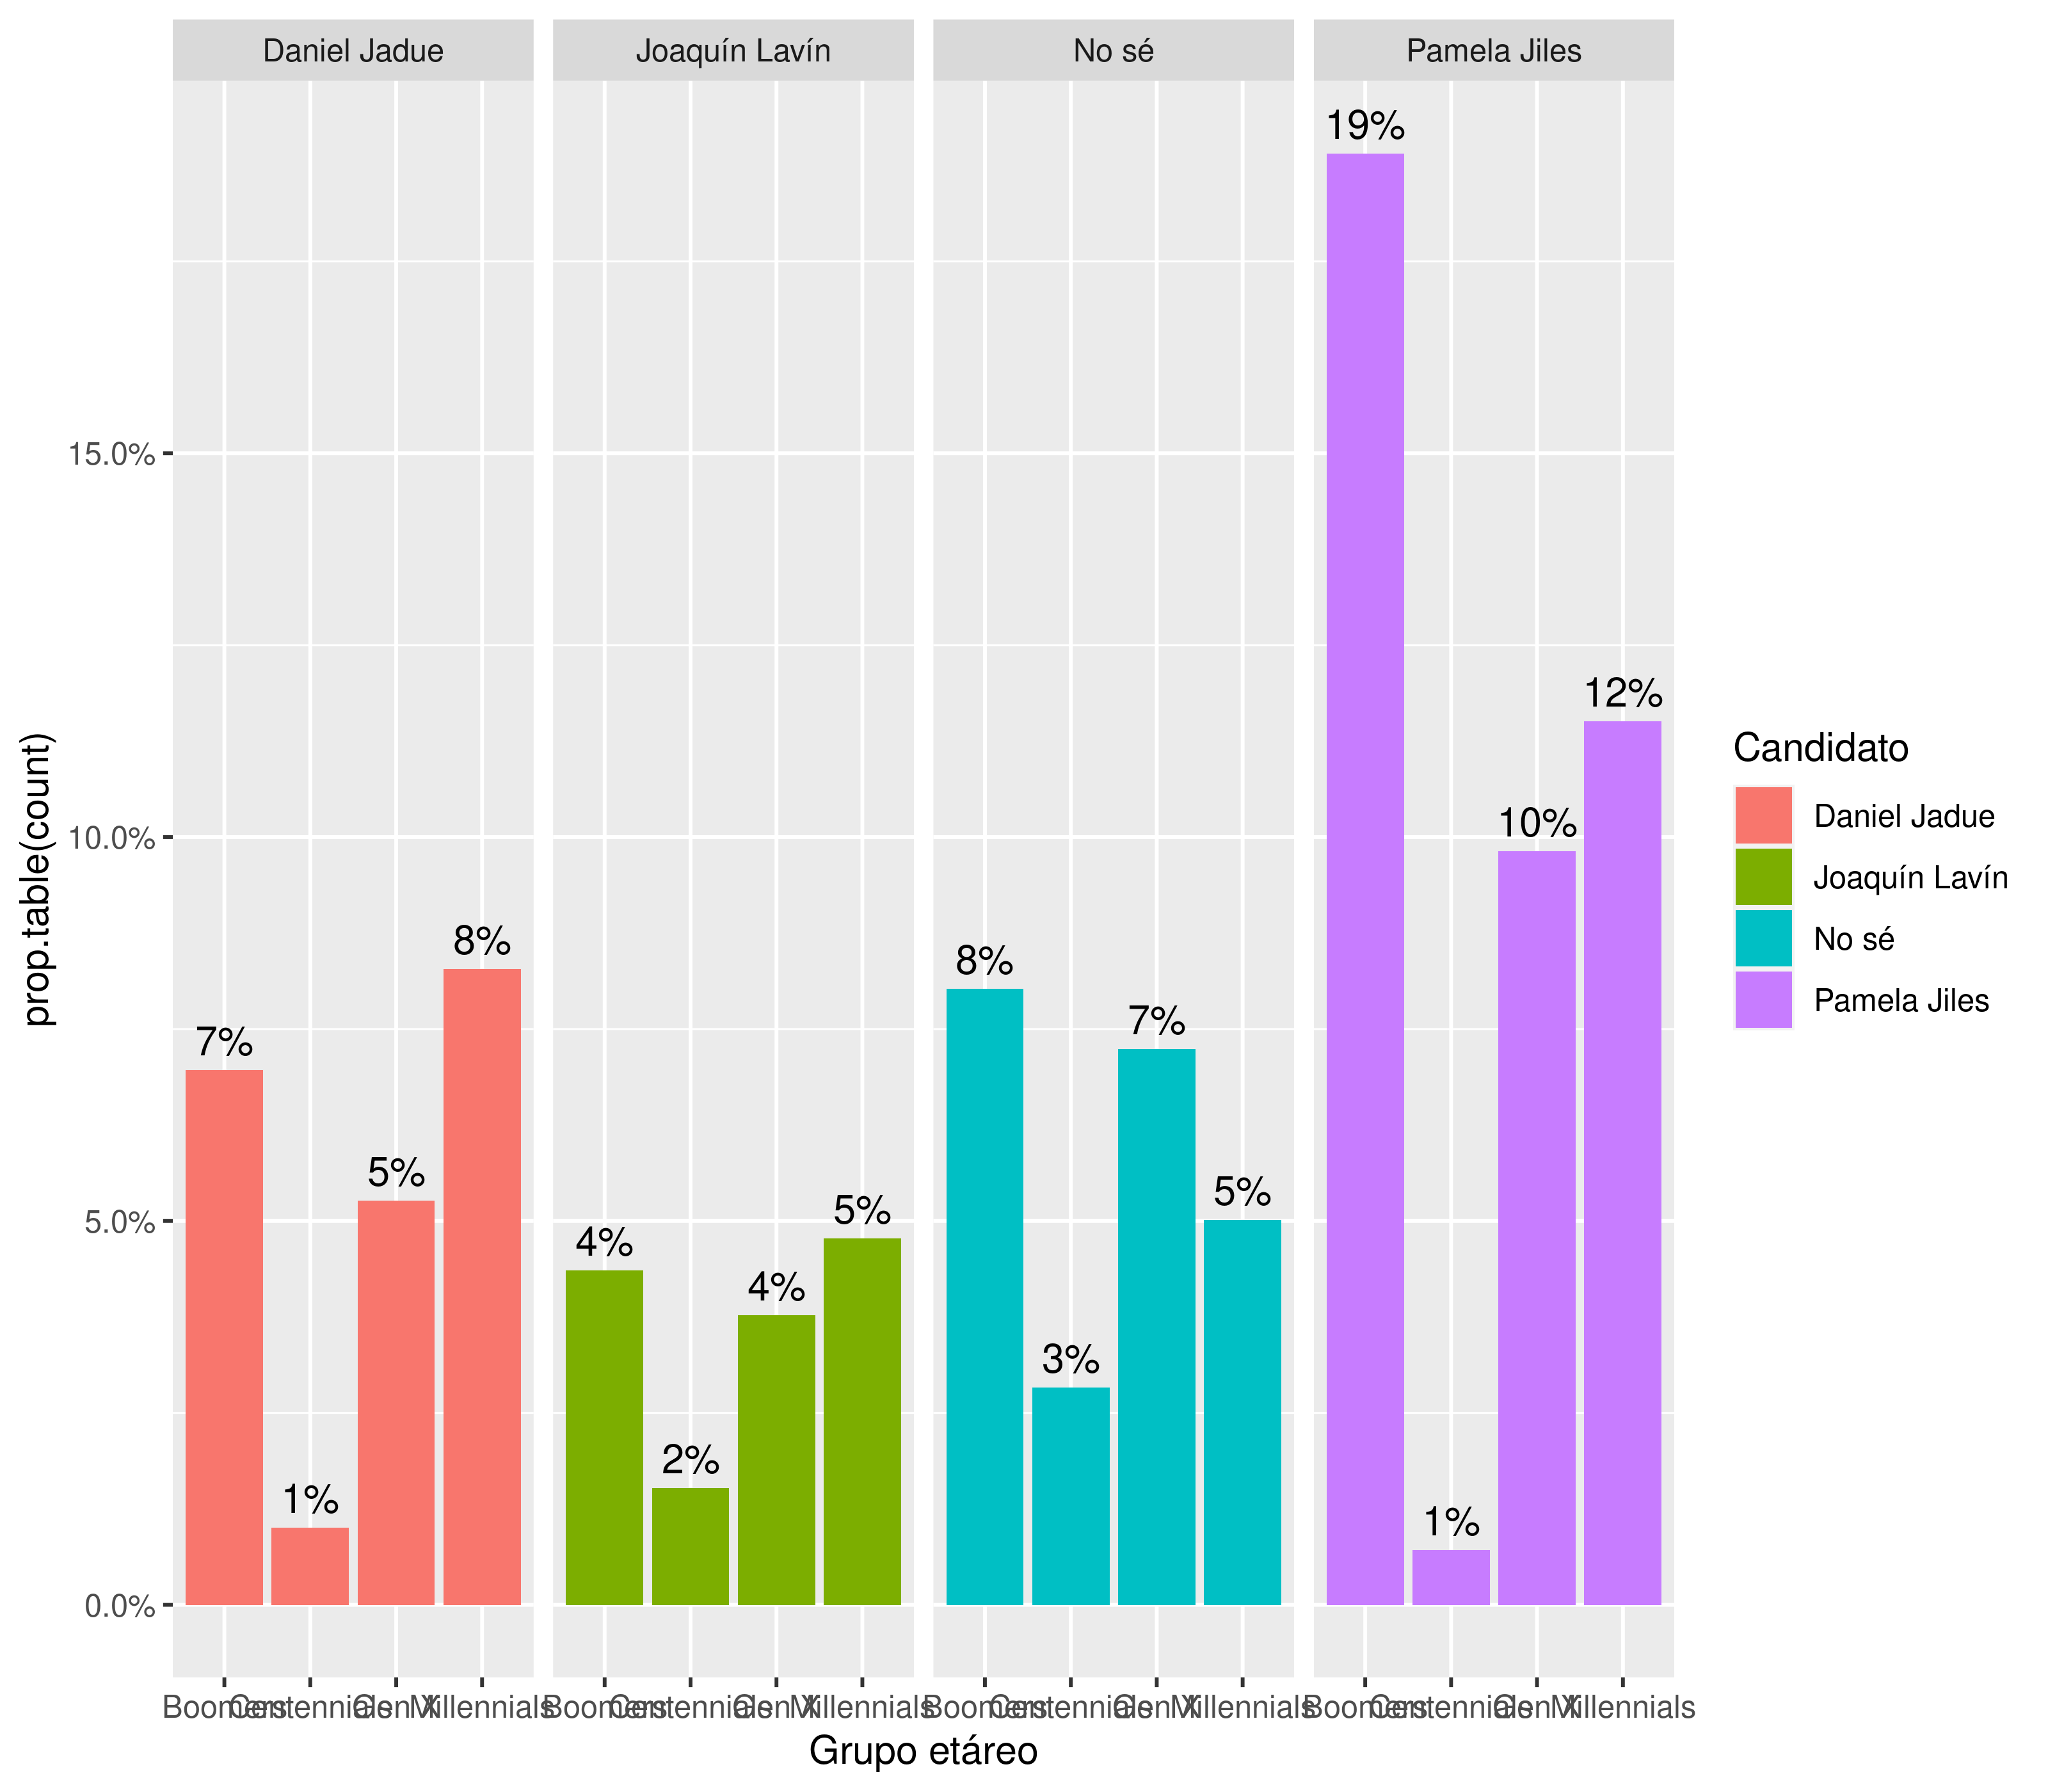
\includegraphics{MoniPlot.png} Lo que se puede decir de esta tabla y
gráfico, y es algo que resaltaremos después en términos electorales, es
que los tipos de votnates de Pamela Jiles y Daniel jadue en este ámbito
exhiben una gran similitud. En ambas candidaturas están con muy
similares porcentajes la cantidad de personas que llegan ``justo'' con
el dinero a fin de mes, así como personas que sencillamente no alcanzan
con el dinero que ganan, lo que se relaciona con lo que anteriormente se
señalaba de los sectores de \emph{trabajadores pobres}

\hypertarget{posiciuxf3n-poluxedtica}{%
\subsection{\texorpdfstring{\textbf{Posición
política}}{Posición política}}\label{posiciuxf3n-poluxedtica}}

La posición política de las personas que papoyan a ciertos candidatos
podría ser un tema baladí en otros períodos de la historia, pero hoy
sobre todo especialmente necesairo observar de qué manera se identifican
políticamente las personas para ver hacia qué sectores el candidato
puede crecer, con quienes pueden hacer alianzas y cómo es percibido por
la población en ausencia de gente con ciertas identificaciones

\newline

\begin{longtable}[]{@{}rrrrrrr@{}}
\toprule
\endhead
\begin{minipage}[t]{0.17\columnwidth}\raggedleft
\strut
\end{minipage} & \begin{minipage}[t]{0.05\columnwidth}\raggedleft
Candi\strut
\end{minipage} & \begin{minipage}[t]{0.12\columnwidth}\raggedleft
Daniel Jadue\strut
\end{minipage} & \begin{minipage}[t]{0.11\columnwidth}\raggedleft
Joaquín Lavín\strut
\end{minipage} & \begin{minipage}[t]{0.12\columnwidth}\raggedleft
No sé\strut
\end{minipage} & \begin{minipage}[t]{0.12\columnwidth}\raggedleft
Pamela Jiles\strut
\end{minipage} & \begin{minipage}[t]{0.12\columnwidth}\raggedleft
Total\strut
\end{minipage}\tabularnewline
\begin{minipage}[t]{0.17\columnwidth}\raggedleft
PosPol\strut
\end{minipage} & \begin{minipage}[t]{0.05\columnwidth}\raggedleft
\strut
\end{minipage} & \begin{minipage}[t]{0.12\columnwidth}\raggedleft
\strut
\end{minipage} & \begin{minipage}[t]{0.11\columnwidth}\raggedleft
\strut
\end{minipage} & \begin{minipage}[t]{0.12\columnwidth}\raggedleft
\strut
\end{minipage} & \begin{minipage}[t]{0.12\columnwidth}\raggedleft
\strut
\end{minipage} & \begin{minipage}[t]{0.12\columnwidth}\raggedleft
\strut
\end{minipage}\tabularnewline
\begin{minipage}[t]{0.17\columnwidth}\raggedleft
Centro\strut
\end{minipage} & \begin{minipage}[t]{0.05\columnwidth}\raggedleft
\strut
\end{minipage} & \begin{minipage}[t]{0.12\columnwidth}\raggedleft
4.8 ( 3.9\%)\strut
\end{minipage} & \begin{minipage}[t]{0.11\columnwidth}\raggedleft
5.5 ( 6.8\%)\strut
\end{minipage} & \begin{minipage}[t]{0.12\columnwidth}\raggedleft
6.3 ( 4.9\%)\strut
\end{minipage} & \begin{minipage}[t]{0.12\columnwidth}\raggedleft
5.5 ( 2.4\%)\strut
\end{minipage} & \begin{minipage}[t]{0.12\columnwidth}\raggedleft
22.2 ( 3.9\%)\strut
\end{minipage}\tabularnewline
\begin{minipage}[t]{0.17\columnwidth}\raggedleft
Centro Derecha\strut
\end{minipage} & \begin{minipage}[t]{0.05\columnwidth}\raggedleft
\strut
\end{minipage} & \begin{minipage}[t]{0.12\columnwidth}\raggedleft
0.4 ( 0.4\%)\strut
\end{minipage} & \begin{minipage}[t]{0.11\columnwidth}\raggedleft
14.8 ( 18.2\%)\strut
\end{minipage} & \begin{minipage}[t]{0.12\columnwidth}\raggedleft
4.5 ( 3.4\%)\strut
\end{minipage} & \begin{minipage}[t]{0.12\columnwidth}\raggedleft
3.2 ( 1.4\%)\strut
\end{minipage} & \begin{minipage}[t]{0.12\columnwidth}\raggedleft
23.0 ( 4.1\%)\strut
\end{minipage}\tabularnewline
\begin{minipage}[t]{0.17\columnwidth}\raggedleft
Centro Izquierda\strut
\end{minipage} & \begin{minipage}[t]{0.05\columnwidth}\raggedleft
\strut
\end{minipage} & \begin{minipage}[t]{0.12\columnwidth}\raggedleft
23.2 ( 19.1\%)\strut
\end{minipage} & \begin{minipage}[t]{0.11\columnwidth}\raggedleft
4.7 ( 5.7\%)\strut
\end{minipage} & \begin{minipage}[t]{0.12\columnwidth}\raggedleft
3.0 ( 2.3\%)\strut
\end{minipage} & \begin{minipage}[t]{0.12\columnwidth}\raggedleft
6.6 ( 2.9\%)\strut
\end{minipage} & \begin{minipage}[t]{0.12\columnwidth}\raggedleft
37.5 ( 6.6\%)\strut
\end{minipage}\tabularnewline
\begin{minipage}[t]{0.17\columnwidth}\raggedleft
Derecha\strut
\end{minipage} & \begin{minipage}[t]{0.05\columnwidth}\raggedleft
\strut
\end{minipage} & \begin{minipage}[t]{0.12\columnwidth}\raggedleft
0.0 ( 0.0\%)\strut
\end{minipage} & \begin{minipage}[t]{0.11\columnwidth}\raggedleft
5.7 ( 7.0\%)\strut
\end{minipage} & \begin{minipage}[t]{0.12\columnwidth}\raggedleft
16.2 ( 12.4\%)\strut
\end{minipage} & \begin{minipage}[t]{0.12\columnwidth}\raggedleft
2.7 ( 1.2\%)\strut
\end{minipage} & \begin{minipage}[t]{0.12\columnwidth}\raggedleft
24.6 ( 4.4\%)\strut
\end{minipage}\tabularnewline
\begin{minipage}[t]{0.17\columnwidth}\raggedleft
Izquierda\strut
\end{minipage} & \begin{minipage}[t]{0.05\columnwidth}\raggedleft
\strut
\end{minipage} & \begin{minipage}[t]{0.12\columnwidth}\raggedleft
32.6 ( 26.9\%)\strut
\end{minipage} & \begin{minipage}[t]{0.11\columnwidth}\raggedleft
0.0 ( 0.0\%)\strut
\end{minipage} & \begin{minipage}[t]{0.12\columnwidth}\raggedleft
16.3 ( 12.5\%)\strut
\end{minipage} & \begin{minipage}[t]{0.12\columnwidth}\raggedleft
48.1 ( 20.8\%)\strut
\end{minipage} & \begin{minipage}[t]{0.12\columnwidth}\raggedleft
97.0 ( 17.2\%)\strut
\end{minipage}\tabularnewline
\begin{minipage}[t]{0.17\columnwidth}\raggedleft
No sé\strut
\end{minipage} & \begin{minipage}[t]{0.05\columnwidth}\raggedleft
\strut
\end{minipage} & \begin{minipage}[t]{0.12\columnwidth}\raggedleft
1.5 ( 1.2\%)\strut
\end{minipage} & \begin{minipage}[t]{0.11\columnwidth}\raggedleft
2.0 ( 2.5\%)\strut
\end{minipage} & \begin{minipage}[t]{0.12\columnwidth}\raggedleft
6.3 ( 4.9\%)\strut
\end{minipage} & \begin{minipage}[t]{0.12\columnwidth}\raggedleft
3.6 ( 1.5\%)\strut
\end{minipage} & \begin{minipage}[t]{0.12\columnwidth}\raggedleft
13.4 ( 2.4\%)\strut
\end{minipage}\tabularnewline
\begin{minipage}[t]{0.17\columnwidth}\raggedleft
Sin posición política\strut
\end{minipage} & \begin{minipage}[t]{0.05\columnwidth}\raggedleft
\strut
\end{minipage} & \begin{minipage}[t]{0.12\columnwidth}\raggedleft
58.9 ( 48.5\%)\strut
\end{minipage} & \begin{minipage}[t]{0.11\columnwidth}\raggedleft
48.7 ( 59.8\%)\strut
\end{minipage} & \begin{minipage}[t]{0.12\columnwidth}\raggedleft
77.7 ( 59.6\%)\strut
\end{minipage} & \begin{minipage}[t]{0.12\columnwidth}\raggedleft
161.3 ( 69.8\%)\strut
\end{minipage} & \begin{minipage}[t]{0.12\columnwidth}\raggedleft
346.5 ( 61.4\%)\strut
\end{minipage}\tabularnewline
\begin{minipage}[t]{0.17\columnwidth}\raggedleft
Total\strut
\end{minipage} & \begin{minipage}[t]{0.05\columnwidth}\raggedleft
\strut
\end{minipage} & \begin{minipage}[t]{0.12\columnwidth}\raggedleft
121.4 (100.0\%)\strut
\end{minipage} & \begin{minipage}[t]{0.11\columnwidth}\raggedleft
81.4 (100.0\%)\strut
\end{minipage} & \begin{minipage}[t]{0.12\columnwidth}\raggedleft
130.4 (100.0\%)\strut
\end{minipage} & \begin{minipage}[t]{0.12\columnwidth}\raggedleft
231.0 (100.0\%)\strut
\end{minipage} & \begin{minipage}[t]{0.12\columnwidth}\raggedleft
564.2 (100.0\%)\strut
\end{minipage}\tabularnewline
\bottomrule
\end{longtable}

Una revisión al gráfico con los totales noes muestra esto:

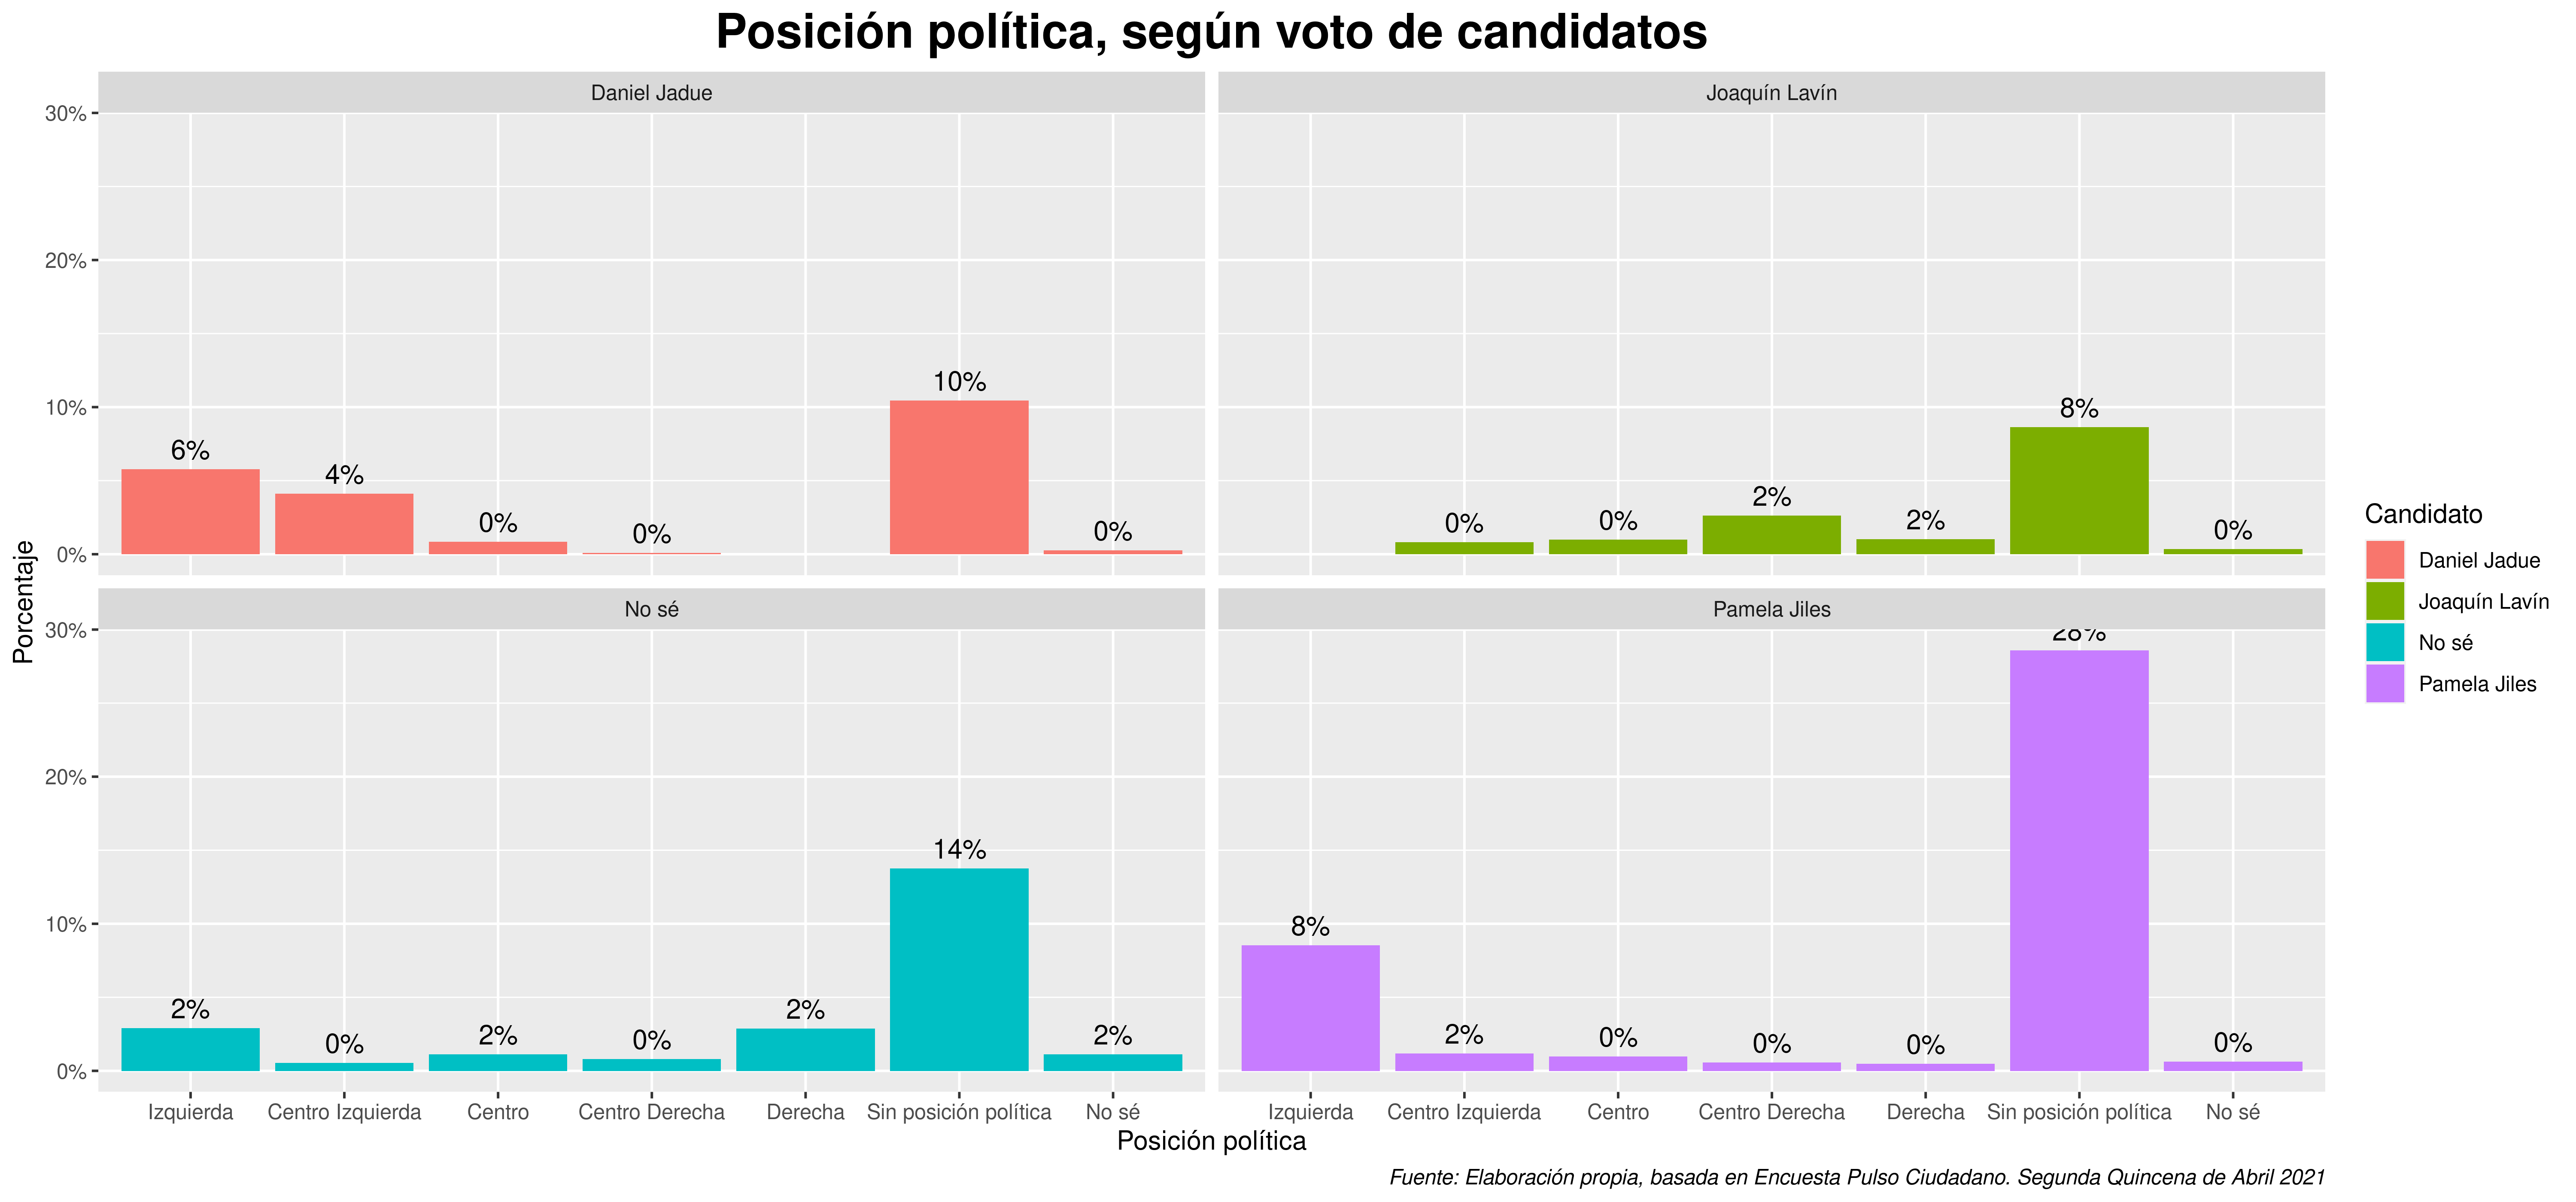
\includegraphics{PolitPlot.png} Uno de los mitos que se han estado
instalando en la prensa (cadem por medio) y en parte de sectores de la
concertación es que Pamela Jiles estaría atrayendo un sector importante
de votos de derecha. Según nuestra investigación esto no es así, y de
hecho sus nichos de identificación política de sus votantes es bastante
clara: casi un 70\% de personas sin identificación política clase, y un
20\% de votantes que se declaran de izquierda. El otro 10\% repartido en
las otras cuatro tendencias donde no hay mucho másque rescatar.

Es interesante esto pues Daniel Jadue, en términos del espectro
ideológico de sus votantes, pareciera ser más conciliador que la propia
Jiles, a pesar del anticomunismo construído de hace décadas en el país.
Vemos que dentro de sus votantes hay casi un 27\% de personas que se
declaran de izquierda, y casi un 20\% de personas de centro izquierda
que votan por él, cuestión inexistente en Jiles. Como contraparte vemos
que jadue llega menos a sectores no identificados ideológicamente, sin
embargo sigue siendo muy algo y rodea el 50\%. Es un candidato
ideológicamente claro al igual que una porción importante de sus
votantes.

En el caso de Joaquín lavín es similar a Jiles pero hacia la derecha:
casi un 60\% de sus votantes declara no tener ideología política
definida, mientras un 18,2\% se declara de ``centro derecha'' y un 7\%
de ``derecha'', porcentaje similar a los que votan por Lavín y se
declaran ``de centro''. Esta ha sido una de las obsesiones del candidato
de la derecha, con el supuesto de que el centro político hace llegar a
más personas, sin embargo los que más hacen llegar a sectores no
ideológicos es quienes no se sienten parte de este eje
izquierda-derecha.

En resumen, Jiles es la que más independiente stiene, a diferencia de
las tesis concertacionistas y de Gamba, no roba muchos votos a la
derecha y Jadue es menos polarizante que Jiles

\begin{longtable}[]{@{}rrrrrrr@{}}
\toprule
\endhead
\begin{minipage}[t]{0.12\columnwidth}\raggedleft
\strut
\end{minipage} & \begin{minipage}[t]{0.06\columnwidth}\raggedleft
Candi\strut
\end{minipage} & \begin{minipage}[t]{0.13\columnwidth}\raggedleft
Daniel Jadue\strut
\end{minipage} & \begin{minipage}[t]{0.12\columnwidth}\raggedleft
Joaquín Lavín\strut
\end{minipage} & \begin{minipage}[t]{0.13\columnwidth}\raggedleft
No sé\strut
\end{minipage} & \begin{minipage}[t]{0.13\columnwidth}\raggedleft
Pamela Jiles\strut
\end{minipage} & \begin{minipage}[t]{0.13\columnwidth}\raggedleft
Total\strut
\end{minipage}\tabularnewline
\begin{minipage}[t]{0.12\columnwidth}\raggedleft
Parti\strut
\end{minipage} & \begin{minipage}[t]{0.06\columnwidth}\raggedleft
\strut
\end{minipage} & \begin{minipage}[t]{0.13\columnwidth}\raggedleft
\strut
\end{minipage} & \begin{minipage}[t]{0.12\columnwidth}\raggedleft
\strut
\end{minipage} & \begin{minipage}[t]{0.13\columnwidth}\raggedleft
\strut
\end{minipage} & \begin{minipage}[t]{0.13\columnwidth}\raggedleft
\strut
\end{minipage} & \begin{minipage}[t]{0.13\columnwidth}\raggedleft
\strut
\end{minipage}\tabularnewline
\begin{minipage}[t]{0.12\columnwidth}\raggedleft
Independiente\strut
\end{minipage} & \begin{minipage}[t]{0.06\columnwidth}\raggedleft
\strut
\end{minipage} & \begin{minipage}[t]{0.13\columnwidth}\raggedleft
45.5 ( 37.5\%)\strut
\end{minipage} & \begin{minipage}[t]{0.12\columnwidth}\raggedleft
58.6 ( 72.0\%)\strut
\end{minipage} & \begin{minipage}[t]{0.13\columnwidth}\raggedleft
65.3 ( 50.1\%)\strut
\end{minipage} & \begin{minipage}[t]{0.13\columnwidth}\raggedleft
140.0 ( 60.6\%)\strut
\end{minipage} & \begin{minipage}[t]{0.13\columnwidth}\raggedleft
309.3 ( 54.8\%)\strut
\end{minipage}\tabularnewline
\begin{minipage}[t]{0.12\columnwidth}\raggedleft
Opositor\strut
\end{minipage} & \begin{minipage}[t]{0.06\columnwidth}\raggedleft
\strut
\end{minipage} & \begin{minipage}[t]{0.13\columnwidth}\raggedleft
75.6 ( 62.3\%)\strut
\end{minipage} & \begin{minipage}[t]{0.12\columnwidth}\raggedleft
10.3 ( 12.7\%)\strut
\end{minipage} & \begin{minipage}[t]{0.13\columnwidth}\raggedleft
47.2 ( 36.2\%)\strut
\end{minipage} & \begin{minipage}[t]{0.13\columnwidth}\raggedleft
85.1 ( 36.8\%)\strut
\end{minipage} & \begin{minipage}[t]{0.13\columnwidth}\raggedleft
218.3 ( 38.7\%)\strut
\end{minipage}\tabularnewline
\begin{minipage}[t]{0.12\columnwidth}\raggedleft
Partidario\strut
\end{minipage} & \begin{minipage}[t]{0.06\columnwidth}\raggedleft
\strut
\end{minipage} & \begin{minipage}[t]{0.13\columnwidth}\raggedleft
0.3 ( 0.3\%)\strut
\end{minipage} & \begin{minipage}[t]{0.12\columnwidth}\raggedleft
12.5 ( 15.3\%)\strut
\end{minipage} & \begin{minipage}[t]{0.13\columnwidth}\raggedleft
17.8 ( 13.7\%)\strut
\end{minipage} & \begin{minipage}[t]{0.13\columnwidth}\raggedleft
6.0 ( 2.6\%)\strut
\end{minipage} & \begin{minipage}[t]{0.13\columnwidth}\raggedleft
36.6 ( 6.5\%)\strut
\end{minipage}\tabularnewline
\begin{minipage}[t]{0.12\columnwidth}\raggedleft
Total\strut
\end{minipage} & \begin{minipage}[t]{0.06\columnwidth}\raggedleft
\strut
\end{minipage} & \begin{minipage}[t]{0.13\columnwidth}\raggedleft
121.4 (100.0\%)\strut
\end{minipage} & \begin{minipage}[t]{0.12\columnwidth}\raggedleft
81.4 (100.0\%)\strut
\end{minipage} & \begin{minipage}[t]{0.13\columnwidth}\raggedleft
130.4 (100.0\%)\strut
\end{minipage} & \begin{minipage}[t]{0.13\columnwidth}\raggedleft
231.0 (100.0\%)\strut
\end{minipage} & \begin{minipage}[t]{0.13\columnwidth}\raggedleft
564.2 (100.0\%)\strut
\end{minipage}\tabularnewline
\bottomrule
\end{longtable}

\begin{longtable}[]{@{}ccc@{}}
\toprule
\begin{minipage}[b]{0.18\columnwidth}\centering
Chi.squared\strut
\end{minipage} & \begin{minipage}[b]{0.06\columnwidth}\centering
df\strut
\end{minipage} & \begin{minipage}[b]{0.13\columnwidth}\centering
p.value\strut
\end{minipage}\tabularnewline
\midrule
\endhead
\begin{minipage}[t]{0.18\columnwidth}\centering
78.0053\strut
\end{minipage} & \begin{minipage}[t]{0.06\columnwidth}\centering
6\strut
\end{minipage} & \begin{minipage}[t]{0.13\columnwidth}\centering
0\strut
\end{minipage}\tabularnewline
\bottomrule
\end{longtable}

Una vista al gráfico nos señala que:

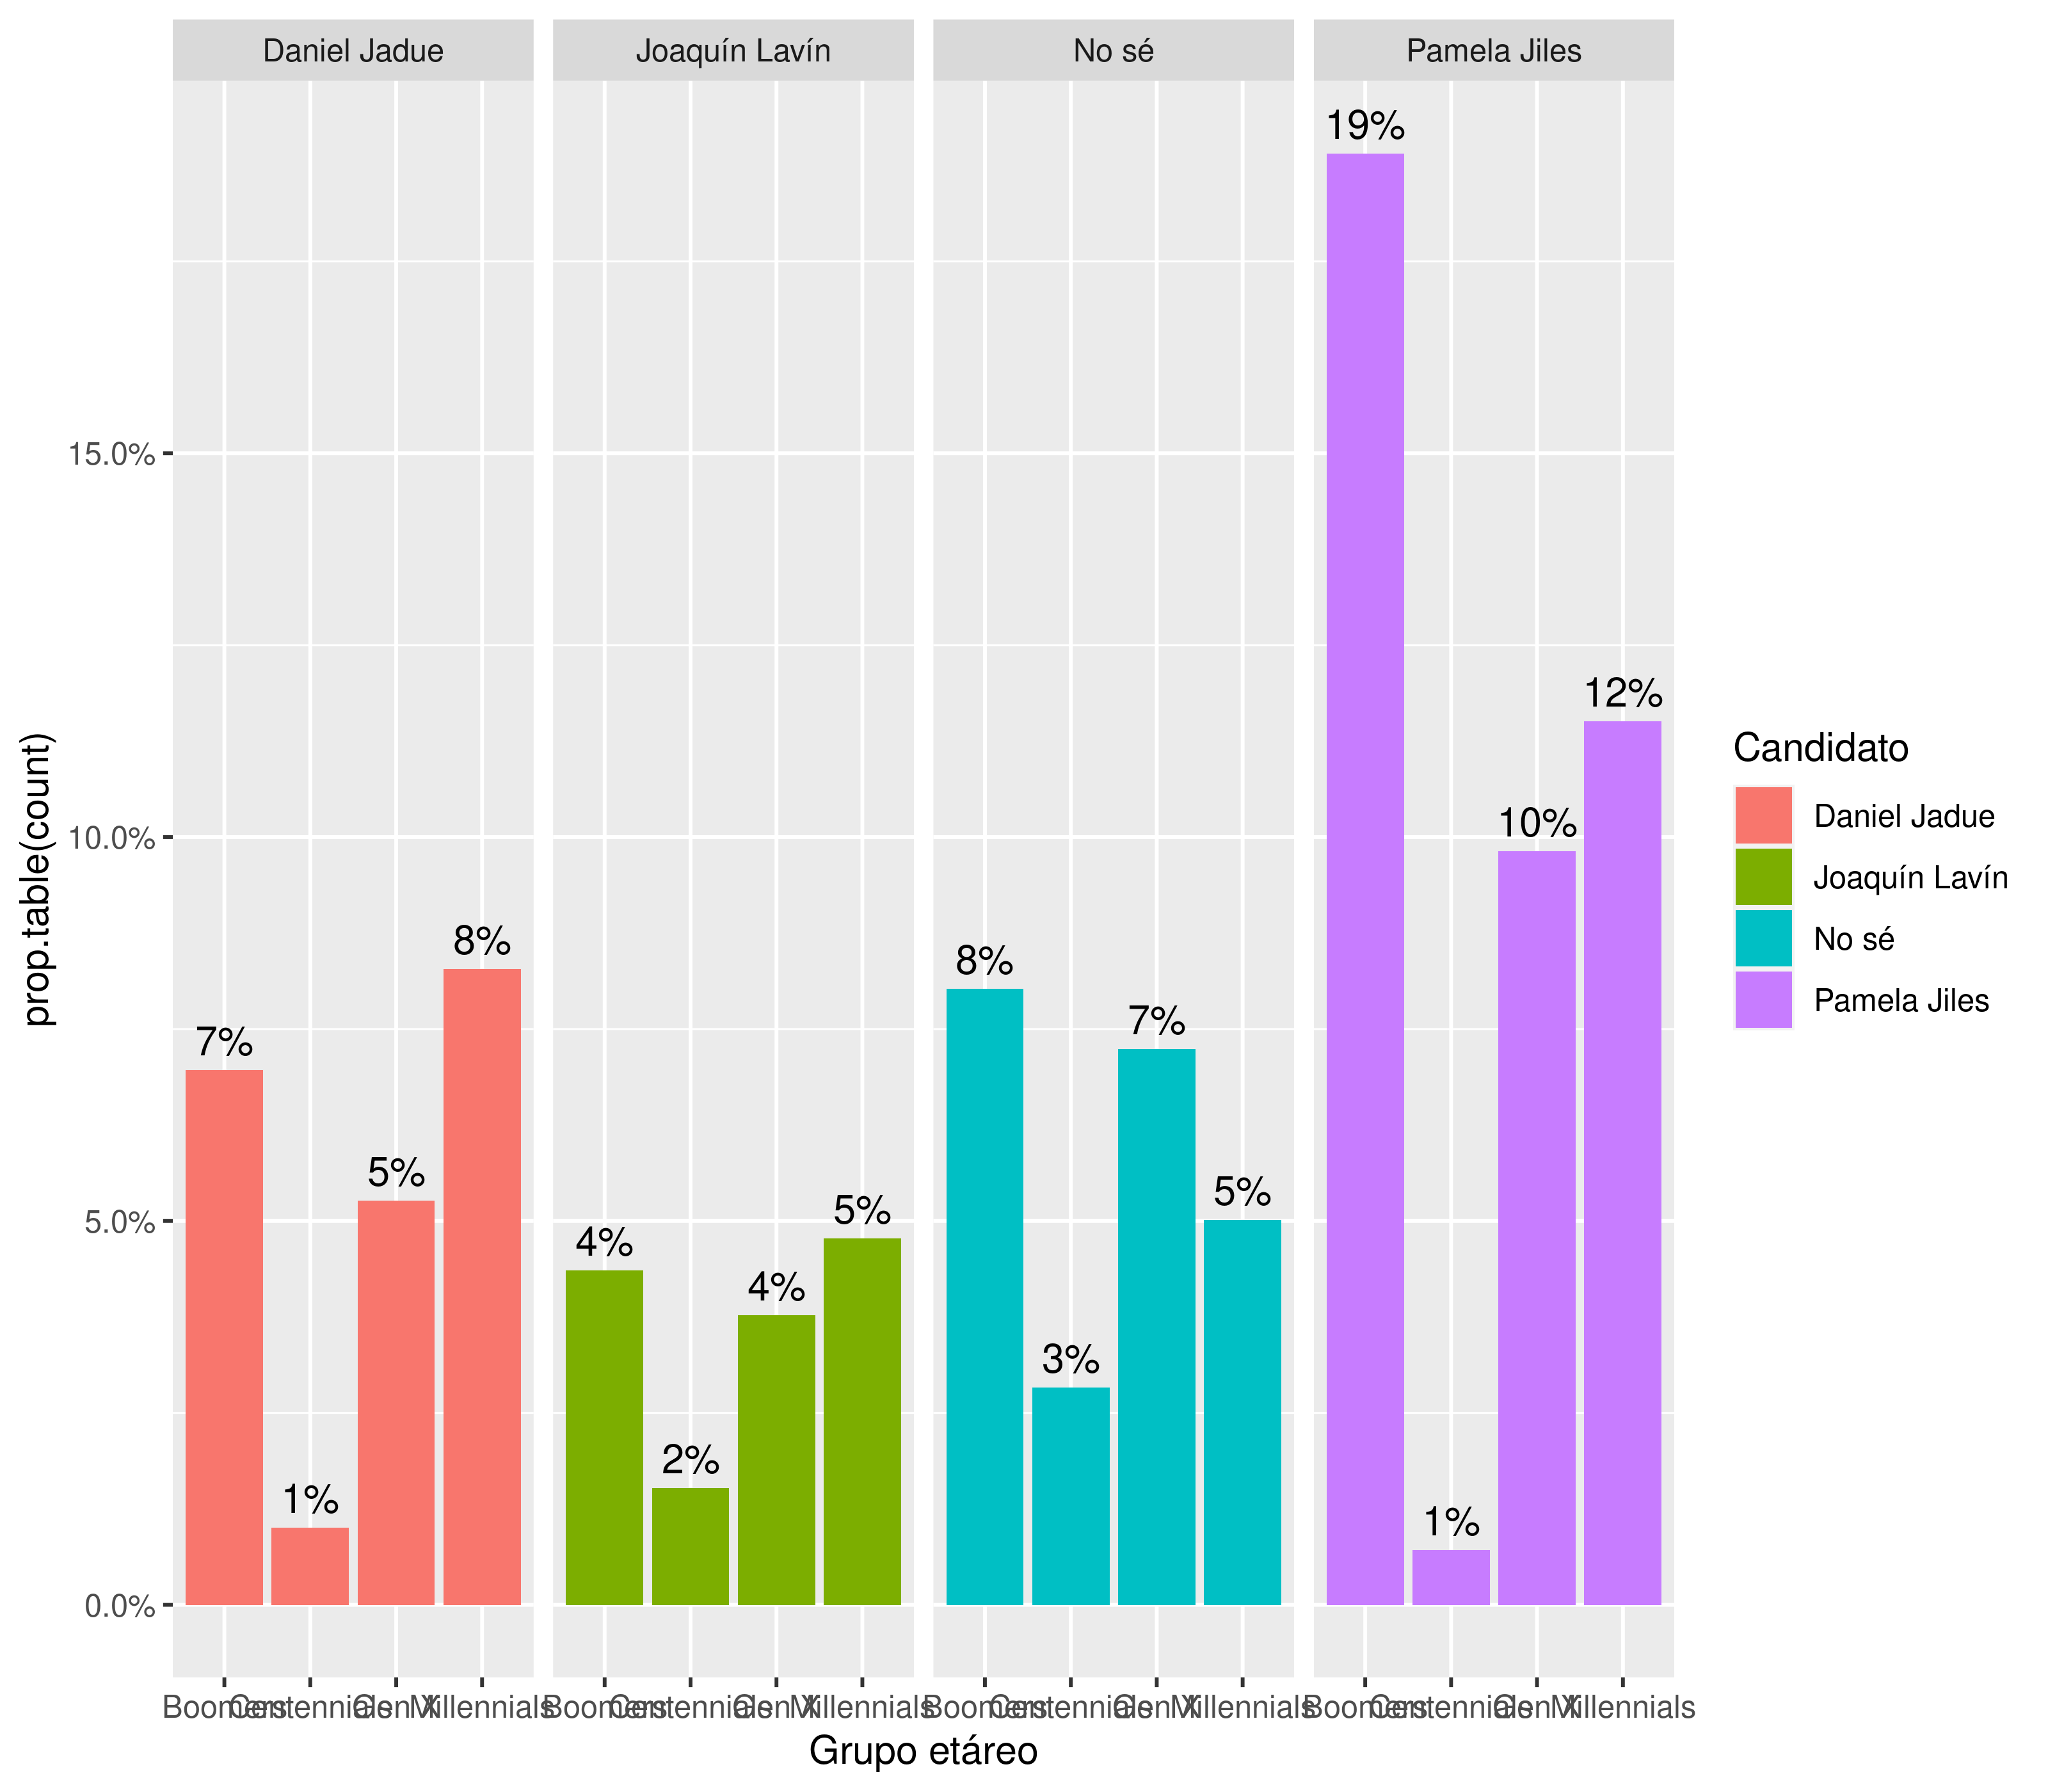
\includegraphics{PartiPlot.png} Esta tendencia se confirma en esta
pregunta, la cuál está diseñada para señalar que uno es independiente en
desmedro a decir que es opositor a Piñera. En este sentido Jiles es la
que más personas ``independientes'' atrase, y Jadue es su absoluto
opuesto, siendo una gran cantidad de sus votantes decididos opositores
al Gobierno de Piñera.

\hypertarget{niveles-de-felicidad}{%
\subsubsection{\texorpdfstring{\textbf{Niveles de
felicidad}}{Niveles de felicidad}}\label{niveles-de-felicidad}}

¿Por qué es importante la felicidad? No importa por sí mjisma, pero los
efectos que tienen las emociones en el comportamiento político son muy
relevantes en la discusión y socialización política, en la forma de
tomar decisiones, en la información a la que yo me expongo (y cuáles
evado) y qué acciones políticas tomaría en el futuro.

Lamentablemente esta encuesta sólo pregunta por niveles de felicidad
habiendo otras emociones relevantes como la ira o el miedo, pero es una
aproximación y hay que tomarla como tal.

Analicemos, pues, el siguiente gráfico:

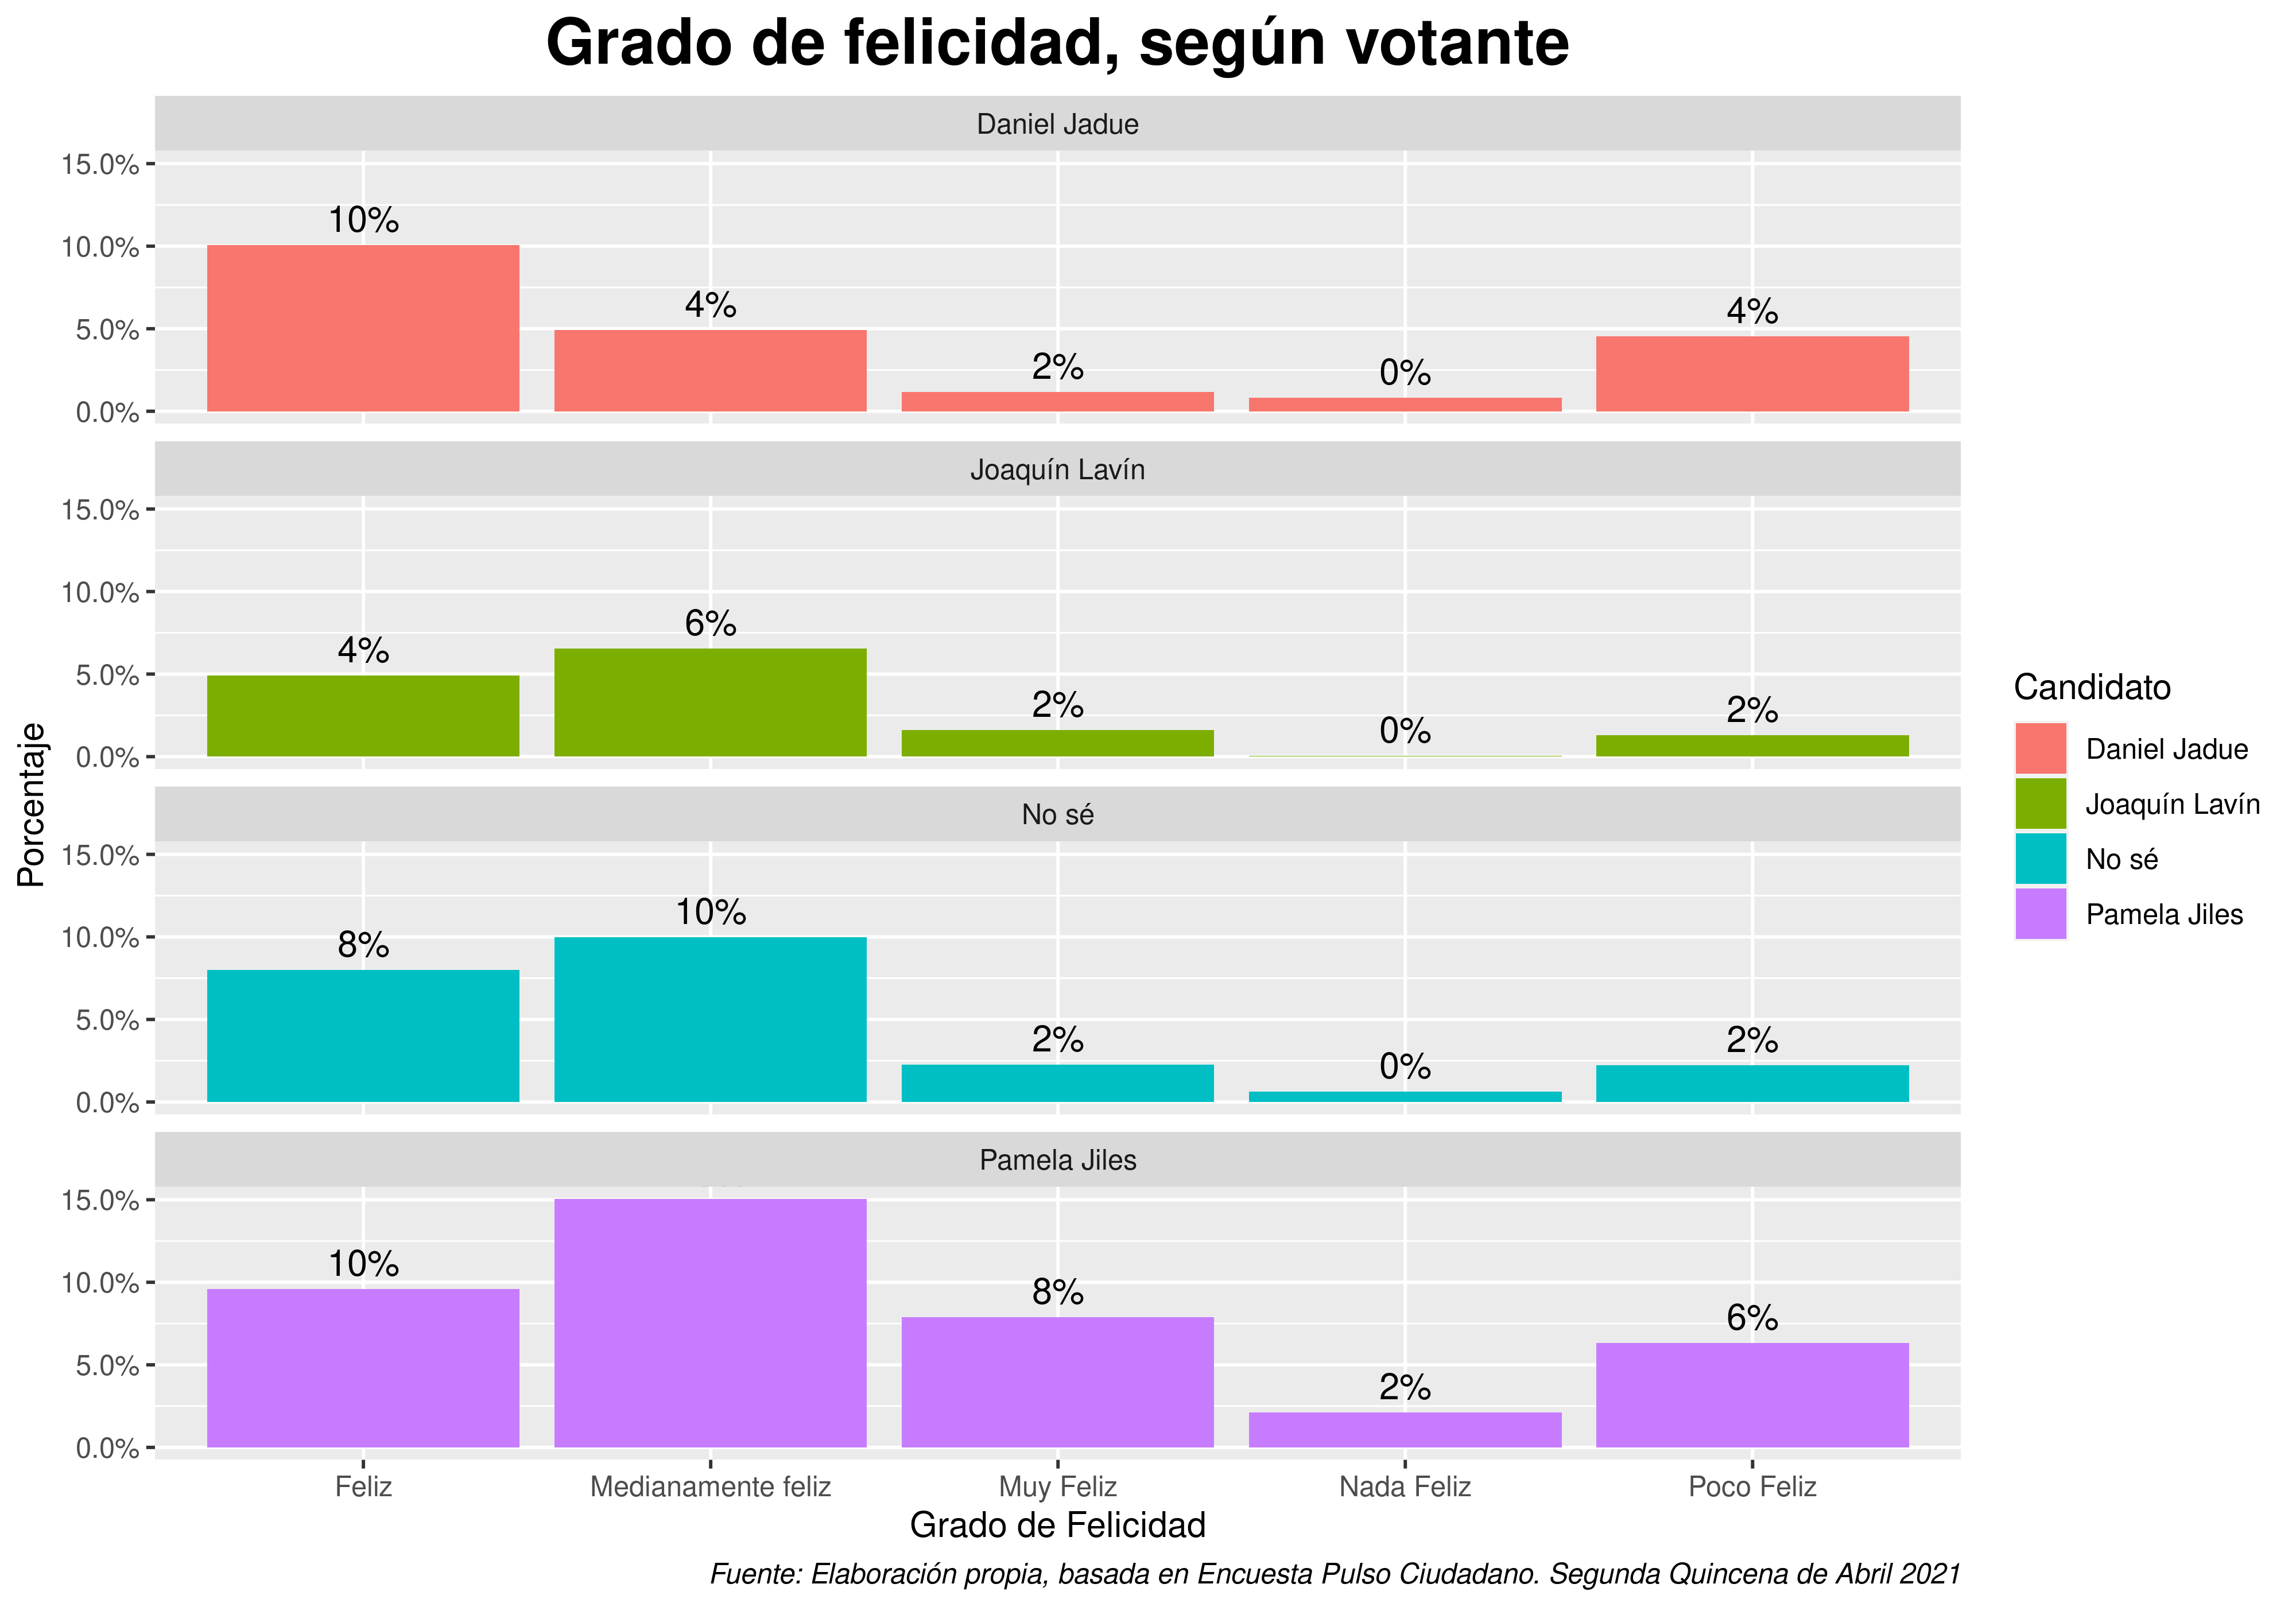
\includegraphics{HappyPlot.png} Este gráfico en principio podría parecer
algo contradictorio en algunos de sus resultados. Primero, los votantes
por Pamela Jiles se reparten principalmente entre Muy felices y
medianamente felices, pero quizás el único gran elemento que vale la
pena analizar son los niveles de ``poco feliz'' y ``nada feliz'', pues
indica que hay otras emociones que pueden estar con niveles de
preponderancia mayores, como enojo, miedo, desesperanza, ansiedad, etc.

De manera unánime, quien lleva las banderas de la poca felicidad son los
votantes de Pamela Jiles, quienes acumulan un 8\% aproximado entre
``nada feliz'' y ``poco feliz''. Se sabe que candidatas radicales que
vienen dsde fuera de loss sistemas políticos explotan emociones como la
ira para generar reputación y empatía con la ciudadanía. Por otro lado
Daniel Jadue es el siguiente que explota esas características, sobre
todo por una tendencia discutsiva antipiñerista que toca teclas
similares a las de Jiles.

\newline

\hypertarget{conclusiones-y-recomendaciones}{%
\subsection{\texorpdfstring{\textbf{Conclusiones y
recomendaciones}}{Conclusiones y recomendaciones}}\label{conclusiones-y-recomendaciones}}

las palabras finales las dividiremos en tres partes esenciales: Perfiles
sociales mayoritarios de cada uno de los candidatos, ``bolsones de
votos'' disponibles según el grupo de indecisos, y por último
recomendaciones a Pamela Jiles y Daniel jadue, ya que son los dos
candidatos por los cuales el autor de este artículo podría eventualmente
adscribir.

\hypertarget{perfiles-de-candidatos}{%
\subsubsection{Perfiles de candidatos}\label{perfiles-de-candidatos}}

\begin{itemize}
\item
  \textbf{Pamela Jiles}: Candidata principal de los Hombres, pobres
  (Cesantes o trabajadores precarizados), principalmente de grupos
  etáreos sobre 40 años en adelante, sobre todo jubilados y mayores de
  52 años´, sin adscripciones ideológicas tan definidas pero aliada
  además de la izquierda y de los detractores de Piñera. Altamente
  polarizante para efectos de posibles alianzas.
\item
  \textbf{Daniel Jadue}: Candidato presidencial de los Hombres,
  trabajadores (De alto nivel como trabajadores precarizados), con gran
  fuerza entre rangos etáreos entre 25 a 50 años, con alta definición
  política con la izquierda y la centro izquierda. Más posibilidad
  conciliadora para alianzas con la centro-izquierda en el caso de
  primarias, pero muy débil para salir más allá de donde ha llegado.
\item
  \textbf{Joaquín lavín}: Candidato presidencial tanto de hombres como
  mujeres, principalmente trabajadores de buena situación económica y de
  las élites, de rango etáreo diverso, con una definición política laxa
  que se traslada al centro político y también a sectores considerados
  independientes. Es probablemente de los candidatos con más amplitud
  para llegar a lugares donde originalmente no llegaba, lo que le
  facilitaría en caso de primarias.
\end{itemize}

\hypertarget{bolsos-de-votos-disponibles}{%
\subsubsection{Bolsos de votos
disponibles}\label{bolsos-de-votos-disponibles}}

Observamos dos grandes bolsones de votos disponibles de personas
indecisas, asumiento que los indecisos son aún más y tienen un
caractertransversal en GSE, sexo, educación, etc. Sin embargo, los
bolsones de votos se centran primero en sectore sjóvenes o Centennialls,
los cuales no tienen ningún referente fuerte del cual poder anclarse.
Otro grupo sumamente abandonado exptresado en los resultados deeste
informe pero también en un análisis político más teórico son las
mujeres. Las personas que han querido llevar las banderas del feminismo
son candidatos que nisiquiera son competitivos, por lo que nisiquiera
son motivo de análisis.

Estos dos grupos pueden dar la victoria definitvia a cualquiera de estos
tres candidatos, o el surgimiento de un cuarto candidato/a igual de
competitivo.

\hypertarget{recomendaciones}{%
\subsubsection{Recomendaciones}\label{recomendaciones}}

\end{document}
